\documentclass[10pt]{beamer}


\mode<presentation> 
{
  \usetheme{Diku}
  \beamertemplatenavigationsymbolsempty
  \setbeamercovered{invisible}
%  \setbeamercovered{transparent}
}



% \usepackage[danish]{babel}
\usepackage[latin1]{inputenc}
\usepackage{times}
\usepackage[T1]{fontenc}
\usepackage[english]{babel}
\usepackage{hyperref}
\usepackage{animate}
%\usepackage{multimedia}
\usepackage{francois-preamble}
\usepackage{multirow}

\usepackage{multirow}
%\usepackage{movie15}

\newcommand{\cc}{{c\!\!,}}
\newcommand{\degr}[1]{{{#1}^\circ}}



\title{Deep learning and CNN's}

\author[S. Olsen] % (optional, use only with lots of authors)
{S�ren Olsen}

\institute[DIKU] % (optional, but mostly needed)
{
  Department of Computer Science\\
  University of Copenhagen
}

\date[2015-16 B1] % (optional, should be abbreviation of conference name)
% {Research Presentation, Diku 2006}


% Insert page numbers
\pagenumbering{arabic}
\setbeamertemplate{footline}{\hspace{5pt}\insertpagenumber\vspace{10pt}}


\definecolor{gold}{rgb}{0.95,0.83,0.0}
\definecolor{orange}{rgb}{0.95,0.7,0.0}
% \definecolor{backblue}{rgb}{0.93,0.94,0.99}
\definecolor{backblue}{rgb}{0.95,0.94,0.99}
\setbeamercolor*{background canvas}{bg=backblue} 



\newcommand{\myemph}[1]{{\color{blue}{#1}}}
\newcommand{\intrg}[1]{\int_{{#1}=-\infty}^\infty}
\newcommand{\intRR}{\int_{-\infty}^\infty}

\AtBeginSection[]
{
  \begin{frame}<beamer>{Outline}
    \tableofcontents[currentsection,currentsubsection]
  \end{frame}
}

\begin{document}
\maketitle




%-------------------------------------------------------------------
%   Start slides
%-------------------------------------------------------------------

% \begin{frame}
%   \frametitle{This ``course''}
% \begin{itemize}
% \item We are a mixed crowd
% \item Today you will have a gentle introduction
% \item The next 2-3-4 weeks we will go into details
% \item You need to self study (i.e. read)
% \item You (not I) is responsible for your progress
% \item Late March, you should plan a midway presentation
% \item In April and May we have less meeting together, but more
%   individual meeting (when you have written part of your report)
% \end{itemize}  
% {\Large
% {\color{blue}{The course evaluation is open until Januar 14}}
% \\[5mm]
% 
% Please fill out the course evaluation.  \\[4mm]
% {\color{red}{It does matter !!!}}
% }
% \end{frame}


%-------------------------------------------------------------------
\begin{frame}
  \frametitle{Today}
  \begin{itemize}
%   \item Please fill out the course evaluation at KUnet.
  \item Litterature and Computer Vision history
  \item Neural nets
  \item Convolutional Neural Nets
  \item CNN Architecture design
  \end{itemize}  
\end{frame}


%-------------------------------------------------------------------
\begin{frame}
  \frametitle{Litterature}
  Ponti et.al. {\em Everything you wanted to know about Deep Learning
    for Computer Vision but were afraid to ask}; 2017 \\[3mm]

  
  \begin{center}
    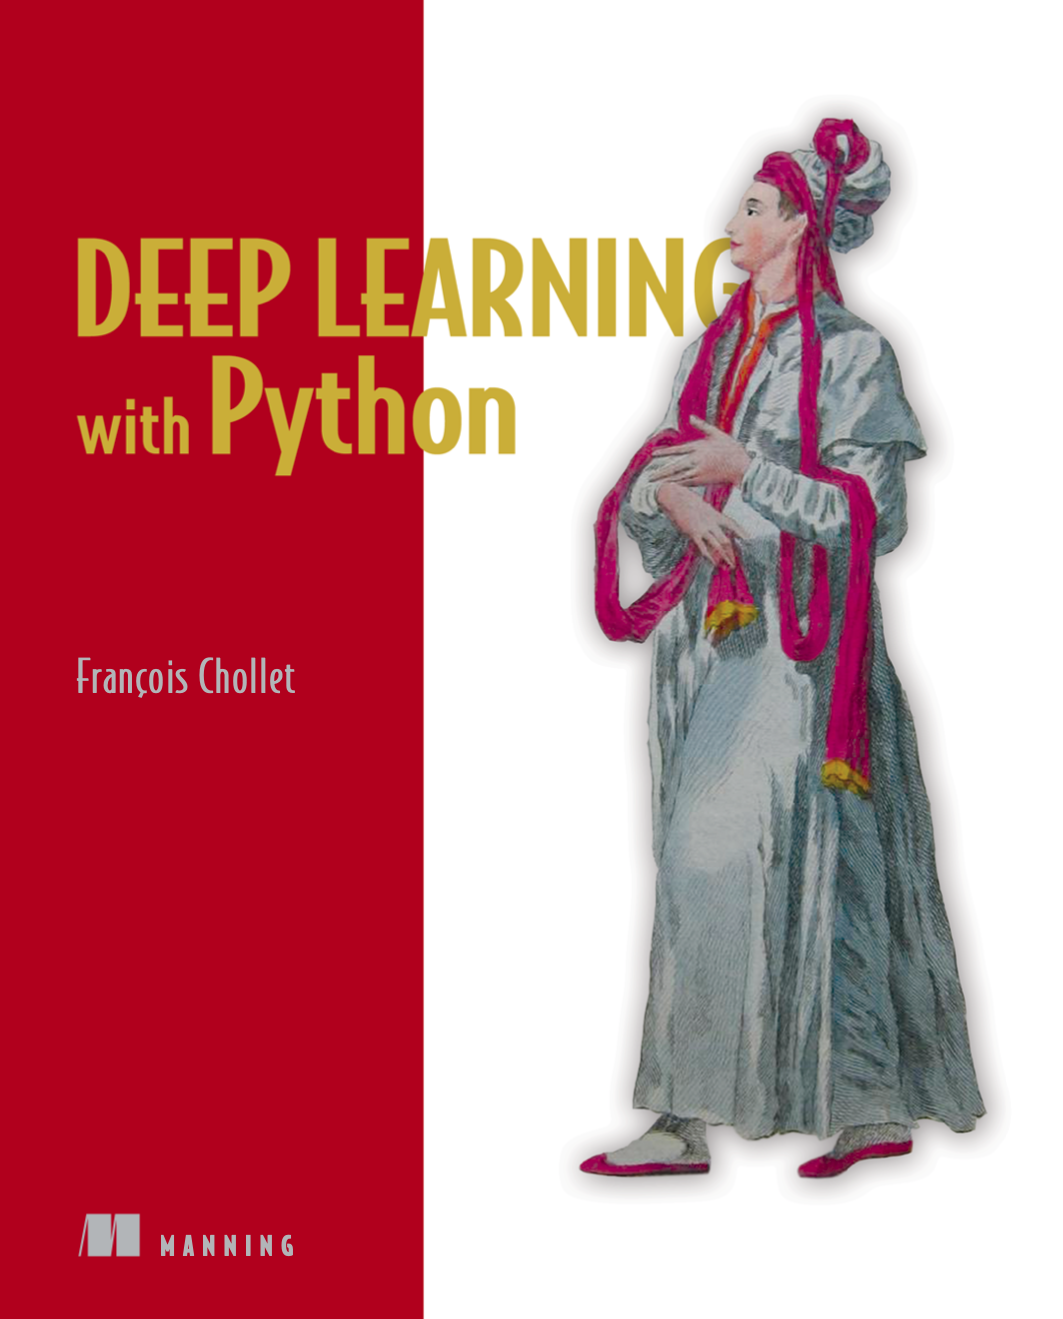
\includegraphics[width=35mm]{Images/Chollet.png}   
    \hspace{2mm}
    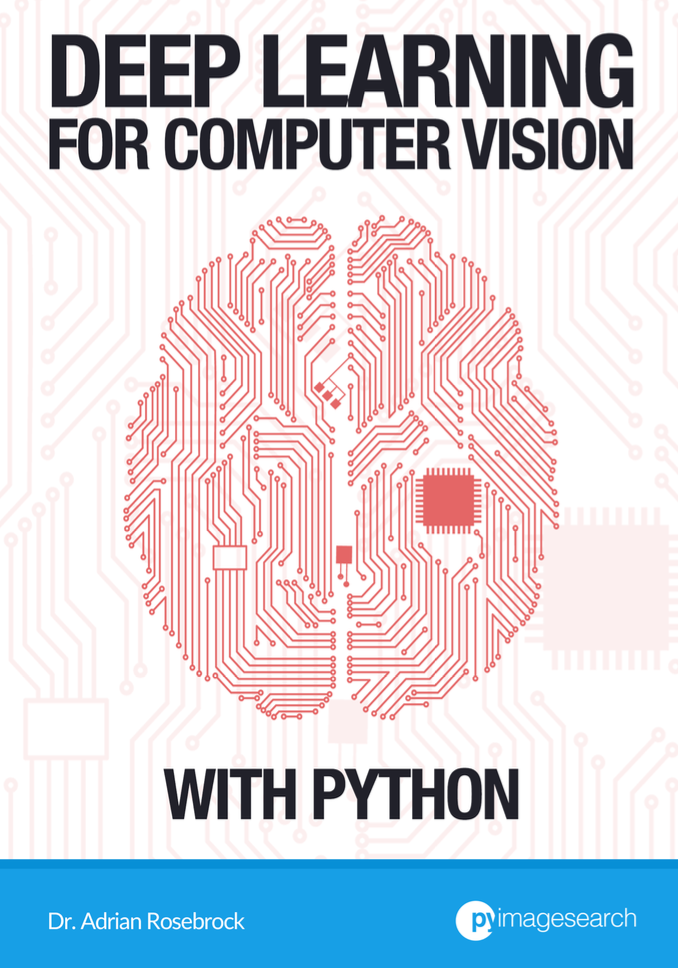
\includegraphics[width=30mm]{Images/Rosenbrock.png}   
    \hspace{2mm}
    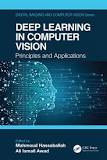
\includegraphics[width=29mm]{Images/DeepLforCV2020.jpg}   
  \end{center}

Liu et.al: {\em A Survey of Convolutional Neural Networks: Analysis,
  Applications and Prospects}; 2021.
\end{frame}



%-------------------------------------------------------------------
\begin{frame}
  \frametitle{IA and AI}

  \begin{center}
    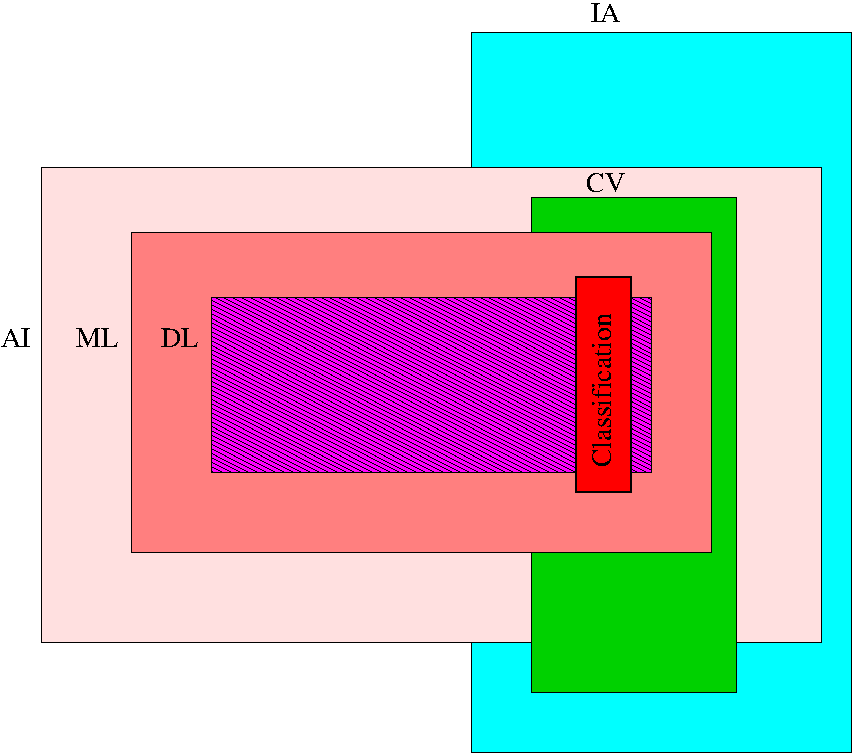
\includegraphics[width=80mm]{Images/IAas.png}   
  \end{center}
\end{frame}



%-------------------------------------------------------------------
\begin{frame}
\frametitle{Background/History} 

Computer Vision (CV) may be viewed as an offspring of 
{\color{blue}{Image processing}}. However, many other disciplines have
played a central role in the development of CV.

\begin{itemize}
\item Computer Science
\item Mathematics
\item Physics (optics)
\item Perceptual psychology
\item Photogrammetry
\item etc.
\end{itemize}
\bigskip

CV is truly multidisciplinary.

\end{frame}



%-------------------------------------------------------------------
\begin{frame}
\frametitle{IP/IA and CV}
Modern image analysis grew up during the 60ies end the 70ies and
matured during the 80ies and 90ies. New methods developed gradually in
parallel with the access to faster and (in particular) larger
computers.
\bigskip

CV developed in USA in the late 70ies.  To some degree a single
person, {\color{blue}{David Marr}} can be credited. Marr was
affilliated with MIT (psychology). In 1980 his book
{\color{blue}{Vision}} gave rise to a burst of research all over the
world. 
\bigskip

Elements of Marr's theory on vision, e.g. the concept of 
{\color{blue}{Scale Space}}, originally suggested by Witkin, may still
be found in many modern approaches and algorithms.

\end{frame}



%-------------------------------------------------------------------
\begin{frame} 
\frametitle{Marr's layers of abstraction}
Marr operate with 3 levels of abstraction following the raw image
data: \\[3mm] 

{\color{magenta}{Primal sketch}} makes explicit features like edges
and blobs, and their spatial geometric relationship, including grouping,
colinearity and terminations. \\[3mm]

{\color{magenta}{2.5D sketch}} represent rough depth of visible
surfaces, discontinuities in depth and orientation all in a viewer
centered coordinate frame. Contributing  processes include
stereo, motion and optical flow, shape from shading etc.\\[3mm]

{\color{magenta}{3D model representation}} describes volumetric
objects and shapes arranged hierarchically in a object centered
coordinate frame. \\[4mm]

Marr imagined a bottom-up process through the layers resulting in an
abstract representation of the 3D scene surrounding us.
\end{frame}



%-------------------------------------------------------------------
\begin{frame} 
\frametitle{The 90ies and the 00s}

This was the golden age of classical CV.  As computers become larger
and faster, new reliable methods emmerged and application began to see
light. In particular within CV, the appropriate mathematics for
expressing e.g. the geometry of multi-view geometry, was established.
\bigskip

A significant development was a number of semi-large databases for
performance measuring of methods for segmentation, stereo, optical
flow, object recognition etc. was created and made public. This
contributed to maturing the field.
\bigskip  

As result, industrial applications became more frequent. Examples
on popular applications include: Google Street View, Shazam, Vivino, 
OCR-systems, Postal code readers, JPG, MPEG, MR-scanner
reconstructions etc. 

\end{frame}



%-------------------------------------------------------------------
\begin{frame} 
\frametitle{Recent trend - Neural nets}
Neural nets have been known since the 40'ies and was (for a few years
during the 90ies) very popular.  However, the models had far too many
unknown parameters, and was far to difficult to train on the available
hardware. Also, essential numerical optimization software and the huge
amount of needed annotated data was not available. \\[4mm]
% \bigskip

In 2012, {\color{blue}{\bf AlexNet}} won the 
{\color{green}{ImageNet Large Scale Visual Recognition Challenge}} by
a large margin over all previous methods.  Alex net was a so-called
{\color{blue}{Convolutional Neural Net}} ({\bf CNN}) with more than 60M
parameters trained on newly available fast
{\color{magenta}{Graphical processing units}} (GPUs) using
{\color{blue}{The backpropagation algorithm}}. \\[6mm]

\begin{center}
{\huge
{\color{red}{\bf This was a game changer}}
}
\end{center}
\end{frame}



%-------------------------------------------------------------------
\begin{frame} 
  \frametitle{ImageNet results}

  \begin{center}
    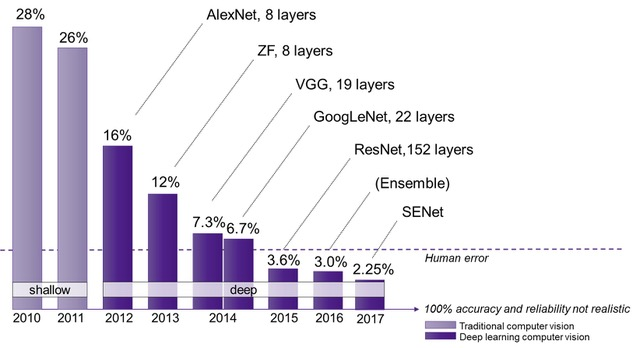
\includegraphics[width=100mm]{Images/ImageNetResults.jpeg}   
  \end{center}

\end{frame}



%-------------------------------------------------------------------
\begin{frame} 
  \frametitle{GPU's}

  \begin{center}
    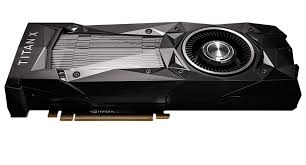
\includegraphics[width=90mm]{Images/titanxp.jpg}   
  \end{center}

  A (now old) Nvidia Titan XP has 3840 Cuda kernels, and delivers about 12
  TFLOPs in processing power. Modern Titan RTX is up to 4 times faster.\\[4mm]

  Popularizing the Cuda platform for parallel programming NVidia has
  established itself as provider of both hardware and low-level
  software for Machine Learning and Image Analysis.
\end{frame}


%-------------------------------------------------------------------
\begin{frame} 
  \frametitle{Backpropagation}

  Neural nets are trained by changing their parameter values such that
  their response becomes closer to the desired output.  This is done
  using (a variant of) {\color{blue}{The backpropagation algorithm}}. \\[6mm]

  First the input is passes through the net and the difference between
  the output and the desired output is computed.  Then, according to a
  specified {\color{blue}{loss-function}}, and using the chain rule of
  differentiation, the errors are passed backwards through the net,
  and the parameters of the neurons adjusted slightly to reduce the
  error. 
  
\end{frame}


%-------------------------------------------------------------------
\begin{frame} 
\frametitle{Automatic differentiation and parallization}

Essential for easy design and use of neural nets is that the updating
equations for the individual parameters in a large net may be
automatically derived and applied. \\[6mm]

Automatic symbolic differentiation has been known for decades and
available in programs such as {\color{blue}{Maple}} and
{\color{blue}{Mathematica}}. During the period 2014-18, a number of
new software platforms spicialized to this task and to application on
a parallel architecture such as a GPU, has emmerged, including:
{\color{blue}{  Caffe, Theano, Torch/Pytorch, Ternsorflow}}. \\[4mm]

Also programming environments, such as {\color{blue}{Keras}} running
on top of the abovementioned makes experimantal implementations easy.
\end{frame}





%-------------------------------------------------------------------
\begin{frame} 
  \vspace{2cm}
  \begin{center}
    {\color{blue}{\huge Questions ?}}
  \end{center}
\end{frame}





%-------------------------------------------------------------------
\begin{frame} 
\frametitle{Neurons}
{\color{blue}{An (artificial) neuron}} is a tiny processing unit that
computes a linear combination of its input values.
\begin{displaymath}
   y \;=\; \sum_i w_i x_i  \;+\, b \;\;=\;\; \sum_j w_j x_j
 \end{displaymath}

\begin{center} 
 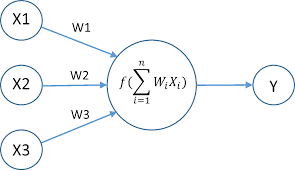
\includegraphics[width=70mm]{Images/nn2.png}   
\end{center}

 {\color{purple}{The simple linear model seems to have very little in common with
neurons found in brains}}. 
%\medskip

\end{frame}



%-------------------------------------------------------------------
\begin{frame} 
\frametitle{Neural Nets} 
For image analysis you may imagine input neurons attached to all
pixels and having all pixel values in a local neighborhood as input.
The net is said to be {\color{blue}{fully connected}}.

\begin{center}
 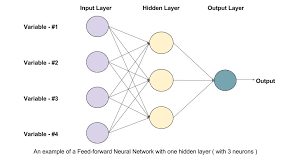
\includegraphics[width=70mm]{Images/nn1.png}   
\end{center}

The 19 parameters (of the toy example above) is not chosen by
engineering/design, but learned. \\[4mm] 

Fully connected nets are expensive in the number of parameters and
often hard to train.  

\end{frame}



%-------------------------------------------------------------------
\begin{frame} 
\frametitle{Convolutional Neural Nets} 
To reduce the number of parameters all neurons within the same layer
may share the same weights $w_i$. In this case the computation will be
a {\color{blue}{convolution}}. \\[5mm]

The basic processing in a CNN is a number of stacked
convolutional layers (CONV). The number of parameters is independent
on the image size, but depend on the number of channels. \\[5mm]

A net with CONV-layers only could be implemented with only a single
layer. To increase the computing repertoire non-linear layers are needed.
\end{frame}





%-------------------------------------------------------------------
\begin{frame} 
\frametitle{Channels}
An RGB-image has 3 channels. The number of input channels to the first
concolutional layer thus is 3.  However, several sub-layers, using the
same input may produce different output and producing a
different/larger number of output channels. \\[5mm]

Usually the number of channels increases (often exponentially) up
through the network. This results in a similar increase in the number of
parameters as we go up through the net. \\[5mm]

It is part of the engineering/design of the network architecture to
choose a small, but sufficient large number of output
filters/channels. This is application dependent.  Often 8-64 are used
at the first layer and the number doubled after each subsampling.

\end{frame}


%-------------------------------------------------------------------
\begin{frame} 
\begin{center}
  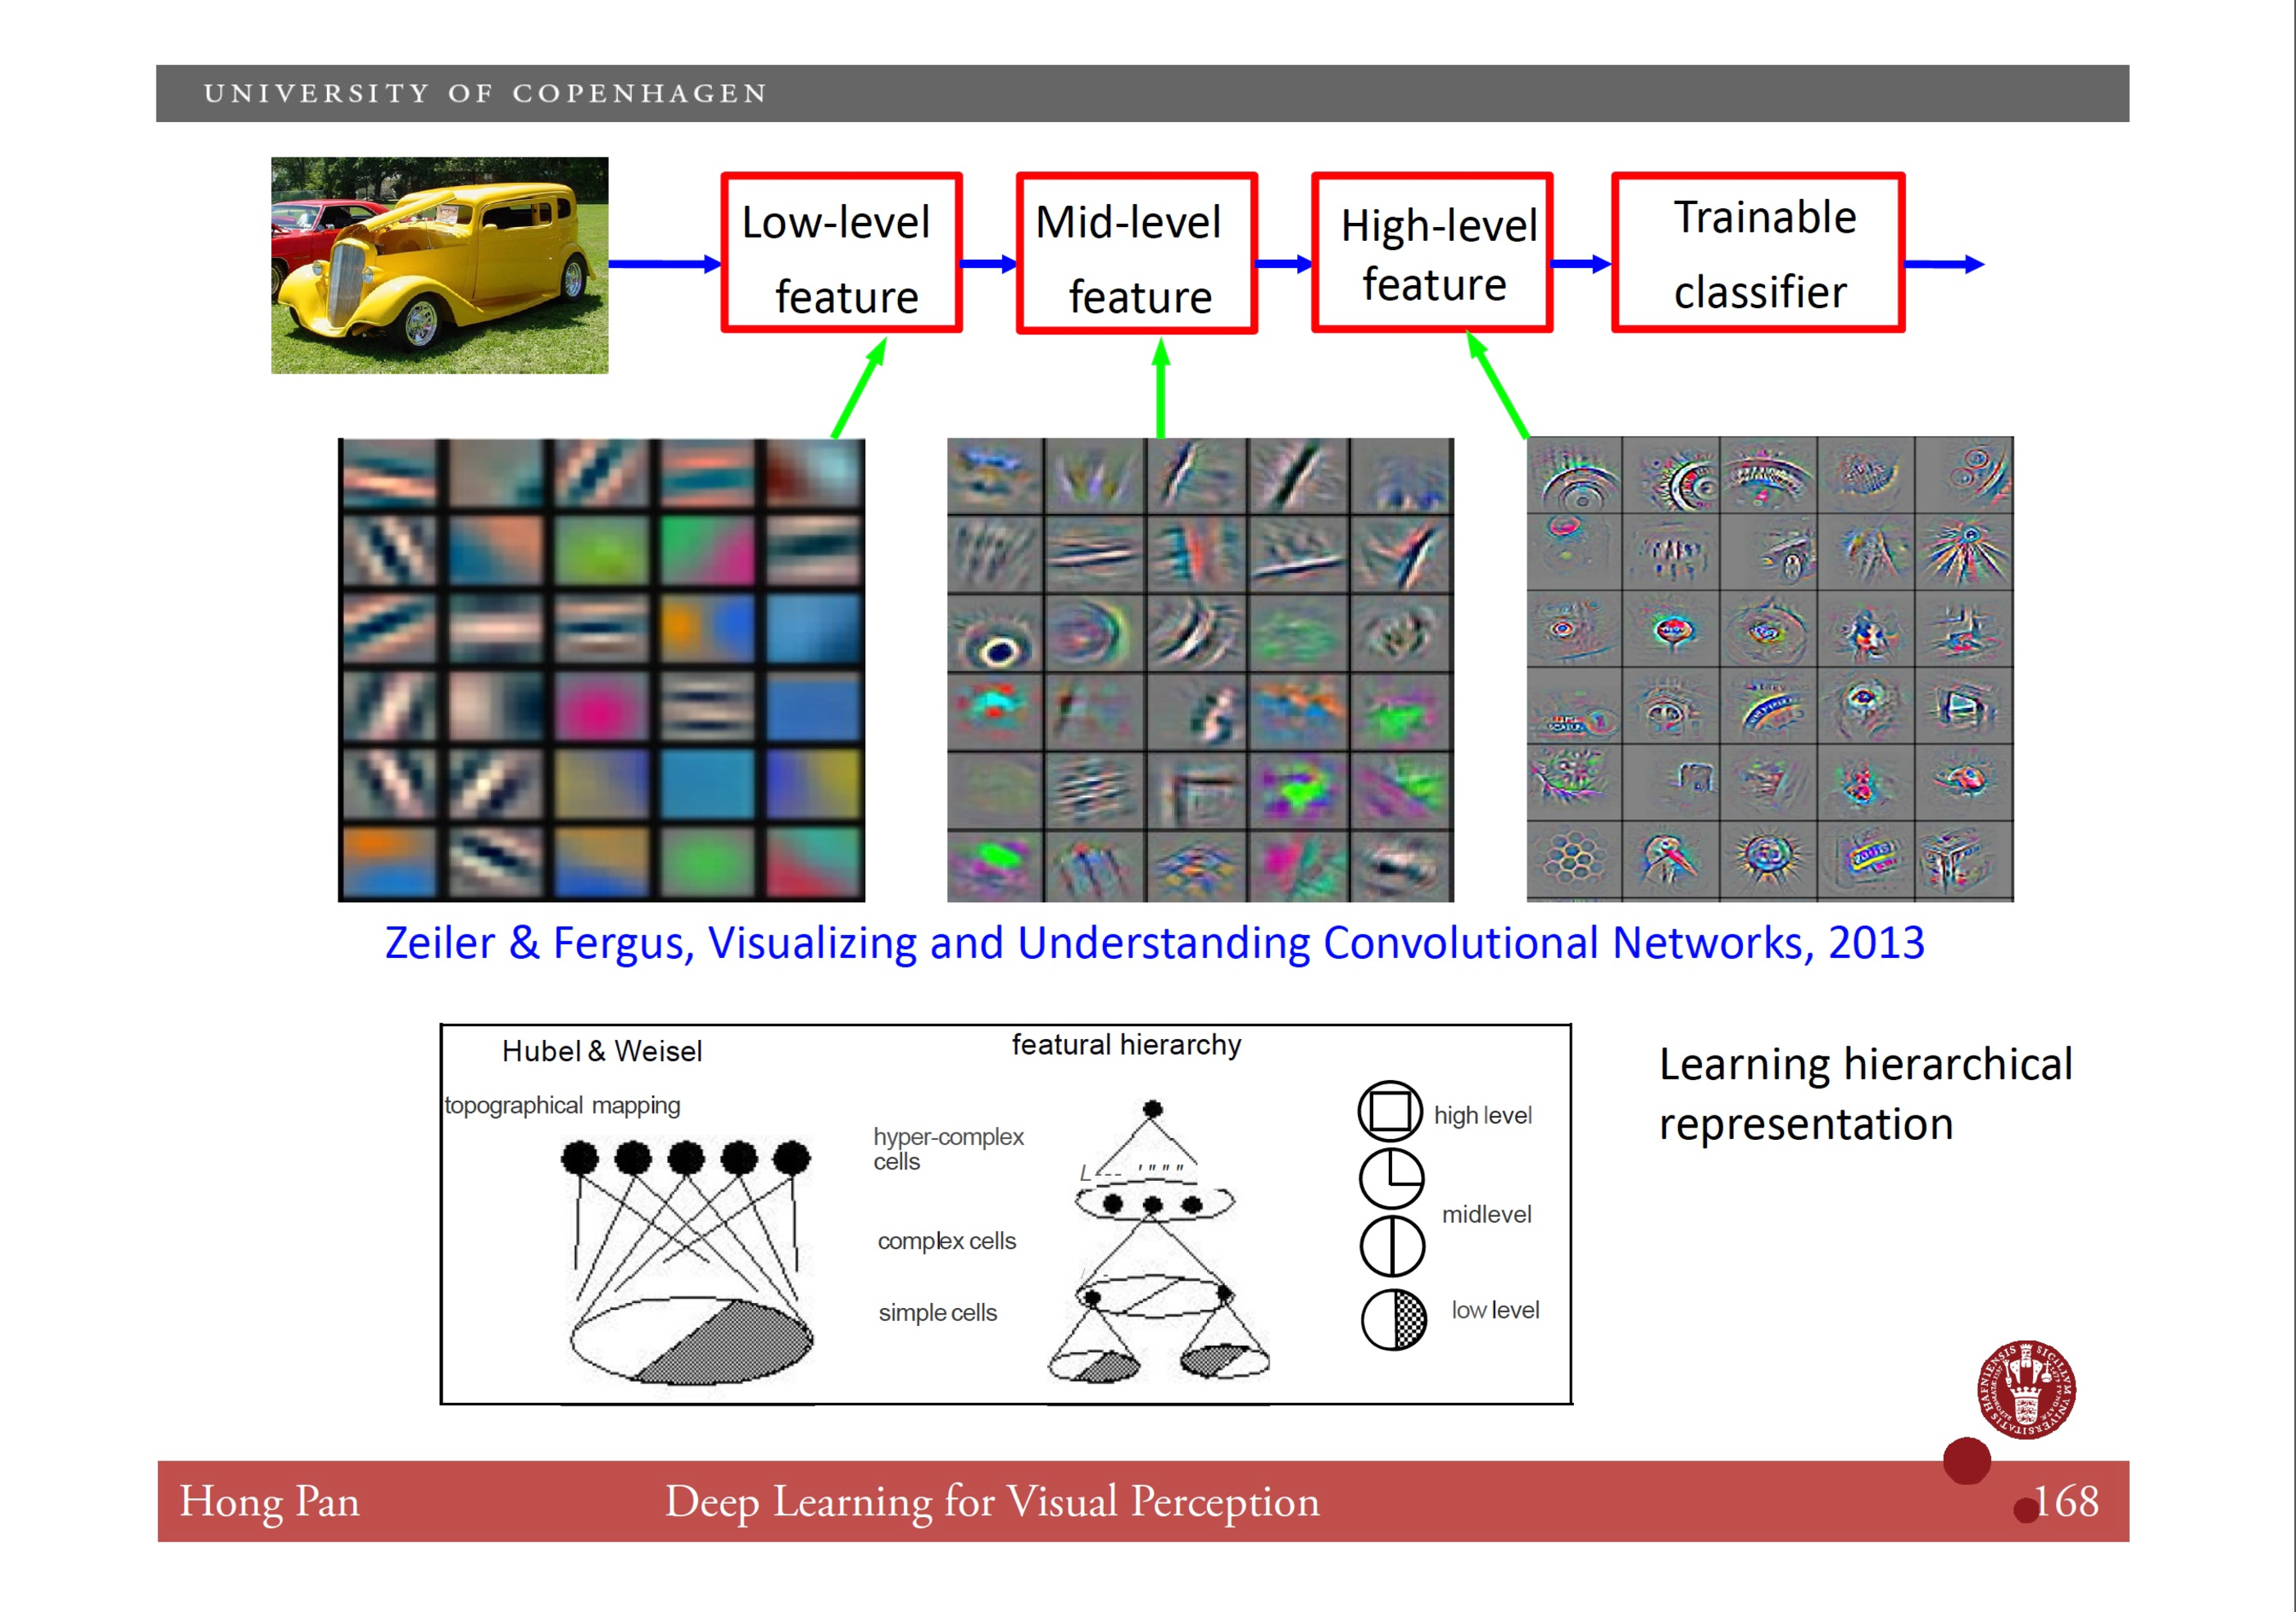
\includegraphics[width=120mm]{Images/FeatureHierarchi.pdf}   
\end{center}
\end{frame}





%-------------------------------------------------------------------
\begin{frame} 
  \frametitle{Convolutions are 3D}
If a filter has a spatial dimension of say $N \times N$ and works on
input with $C$ channels, then the number of parameters are $C N^2
+1$.  \\[2mm]

A 3D kernel (filter) $w_{i,j,c}$ is called a {\color{red}{tensor}}. \\[2mm]

\begin{displaymath}
 y = \sum_i^N \sum_j^N \sum_c^C w_{i,j,c} x(i,j,c) \;+\; b
\end{displaymath}
\bigskip

Thus, a $1 \times 1$ filter is just a pixelwise linear combination of
the channel data. 
\end{frame}




%-------------------------------------------------------------------
\begin{frame} 
\frametitle{Class exercise - 0.5 minute}
\vspace{1cm}
{\Large What math can be computed by $n$-layers of convolutions
  (without any activation function) ?}   

\end{frame}




%-------------------------------------------------------------------
\begin{frame} 
\begin{center}
  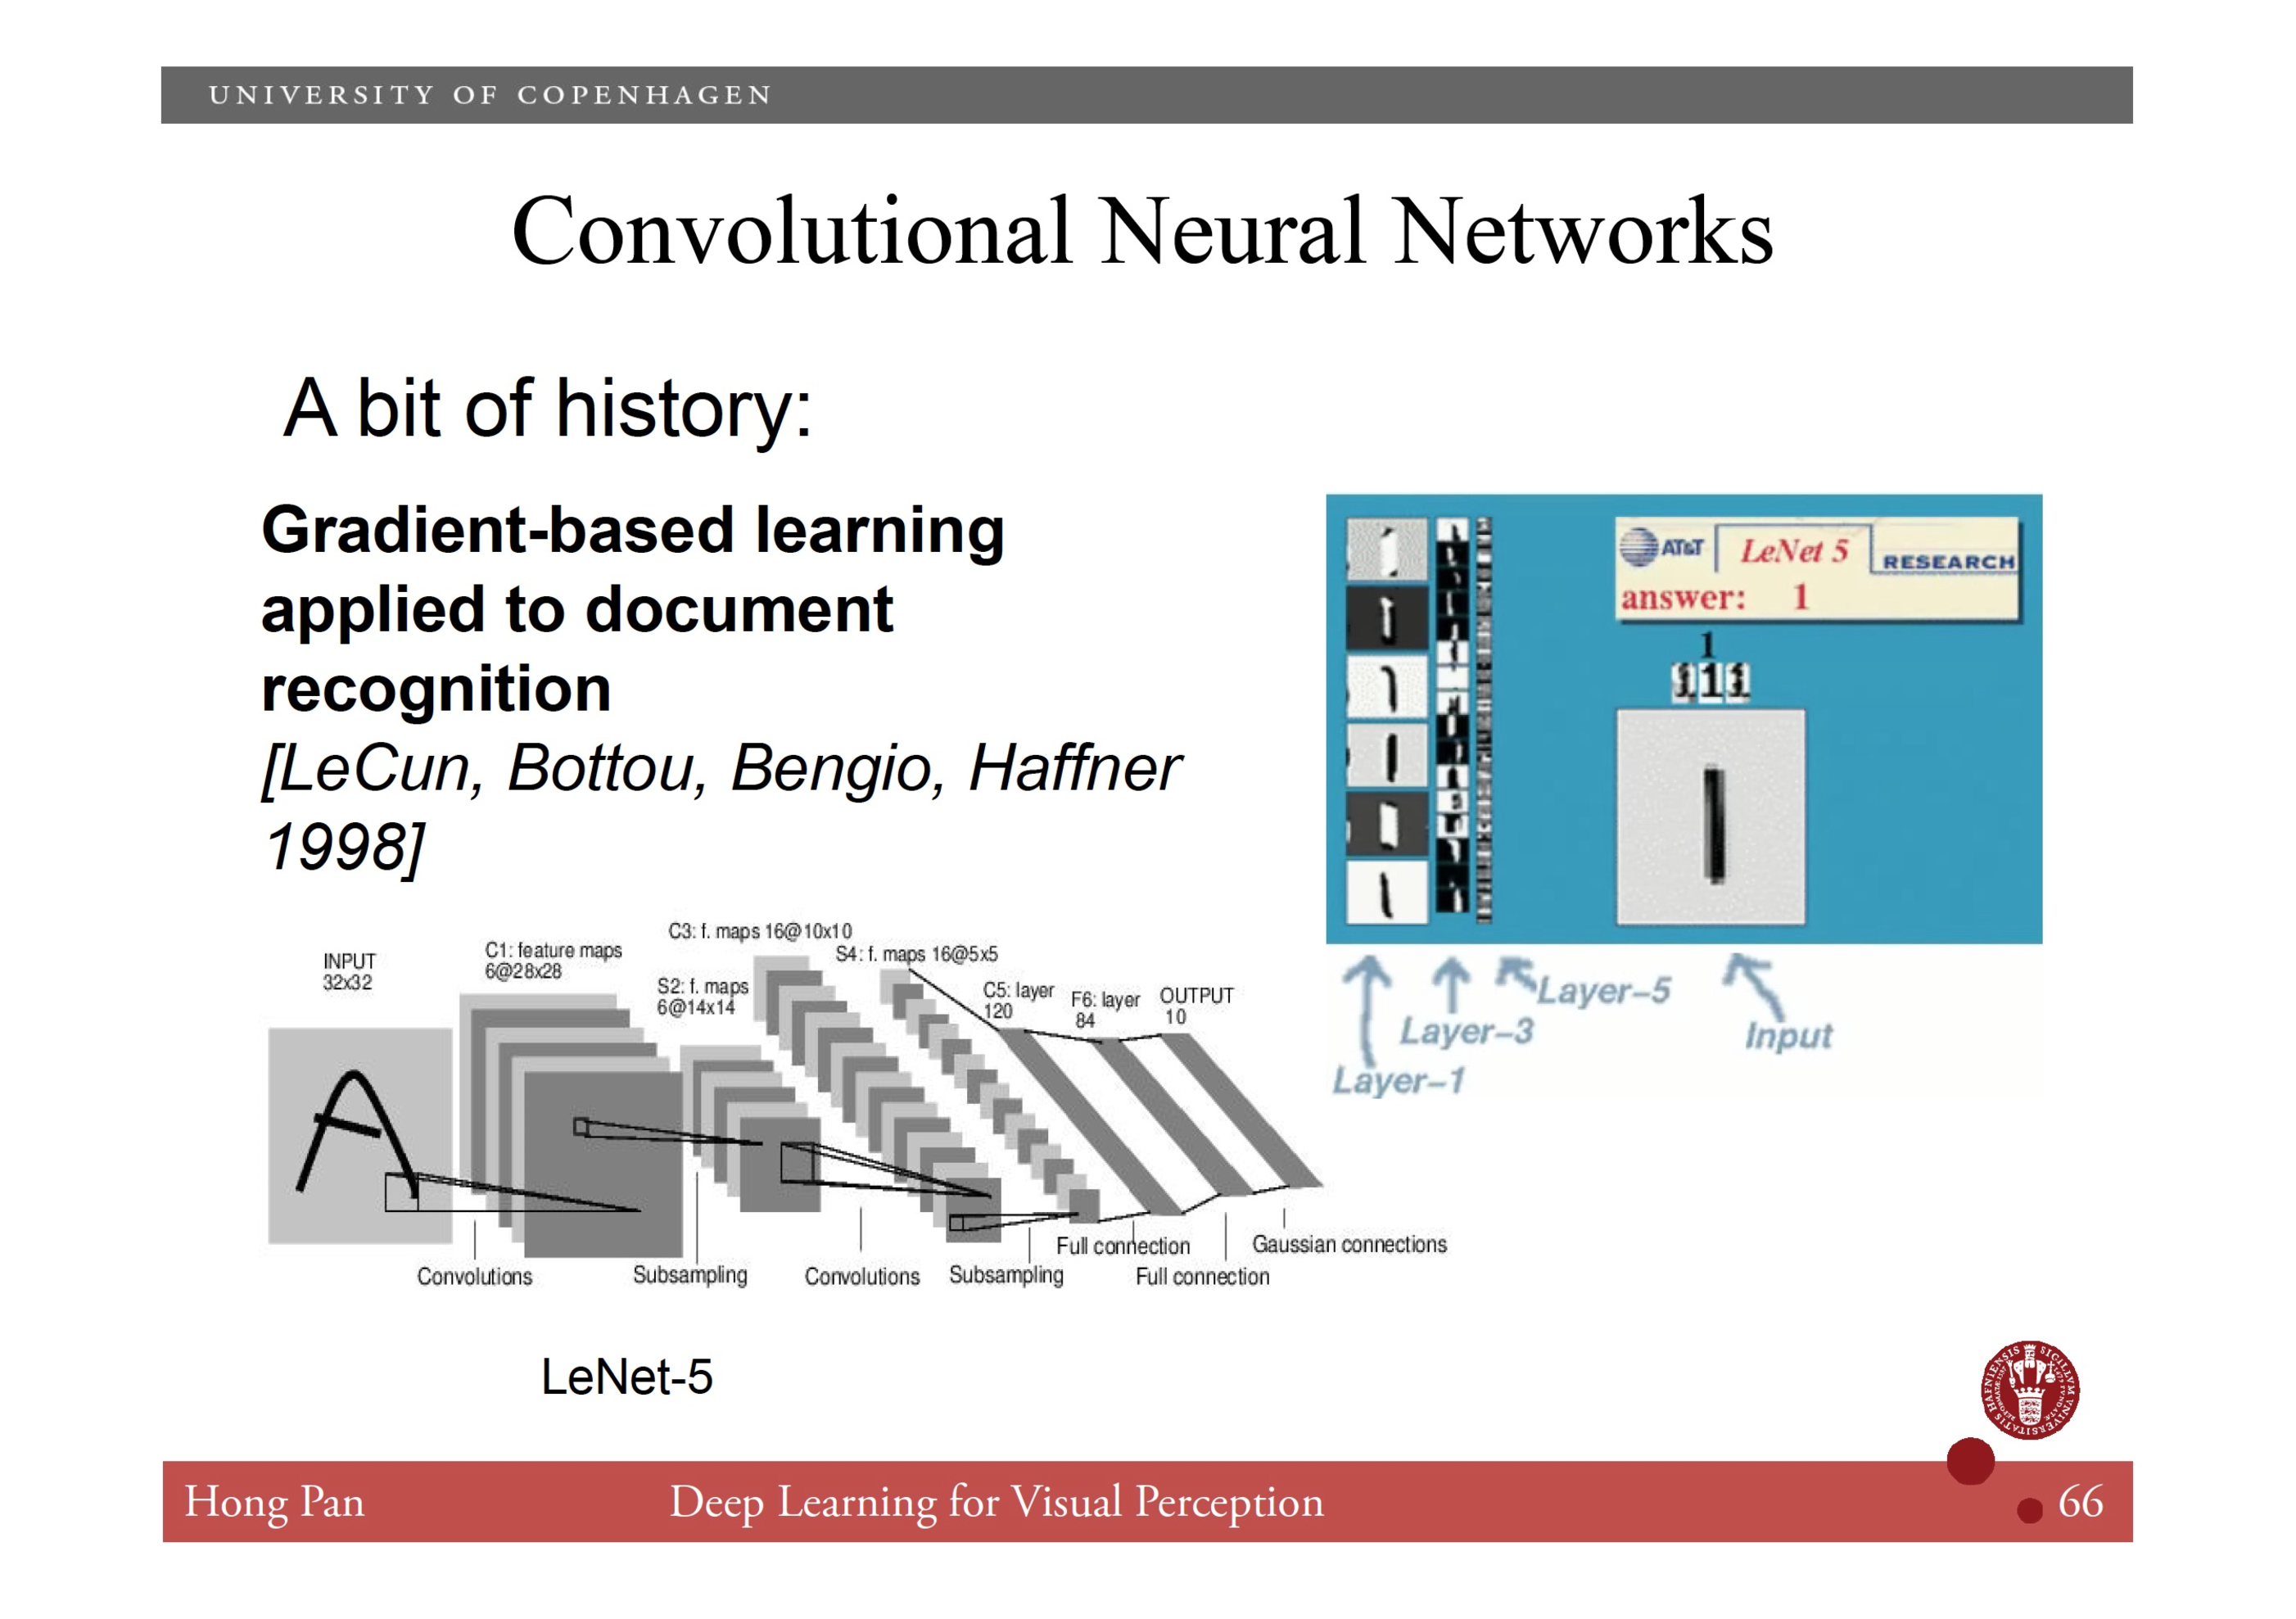
\includegraphics[width=120mm]{Images/CNNex.pdf}   
\end{center}
\end{frame}



%-------------------------------------------------------------------
\begin{frame} 
\frametitle{RELU's}
If the net consisted of convolutional layers only, the final output
would be a convolution.  To increase the functionality, a non-linear
operation is needed. Many has been tried, RELU's have shown superior.  
\bigskip

A RELU ({\color{blue}{REctified Linear Unit}}) is a simple non-linear
operation with no parameters:

\begin{displaymath}
   y \;=\; \left \{ \begin{array}{l l}
         x & \mbox{if $x > 0$} \\ 0 & \mbox{otherwise}
         \end{array}   \right .
\end{displaymath}

Often RELU's are used after each convolutional layer (or after a
sequence of such). 

\end{frame}



%-------------------------------------------------------------------
\begin{frame} 
\frametitle{Class exercise - 0.5 minute}
\vspace{1cm}
{\Large Why do you think a RELU is a (huge) computational advantage
  compared to e.g. a sigmoid ( = $\frac{e^x}{1 + e^x}$)  ?}
\pause
\bigskip

Remember the {\color{blue}{Back-propagation}} algorithm.  What happens
when we differentiate a RELU:

\begin{displaymath}
   y \;=\; \left \{ \begin{array}{l l}
         x & \mbox{if $x > 0$} \\ 0 & \mbox{otherwise}
         \end{array}   \right .
\end{displaymath}

\end{frame}





%-------------------------------------------------------------------
\begin{frame} 
  \frametitle{Leaky RELU}
A Leaky RELU does not map all negative values to zero, but let a tiny
fraction pass. \\[3mm]
  
\begin{center}
  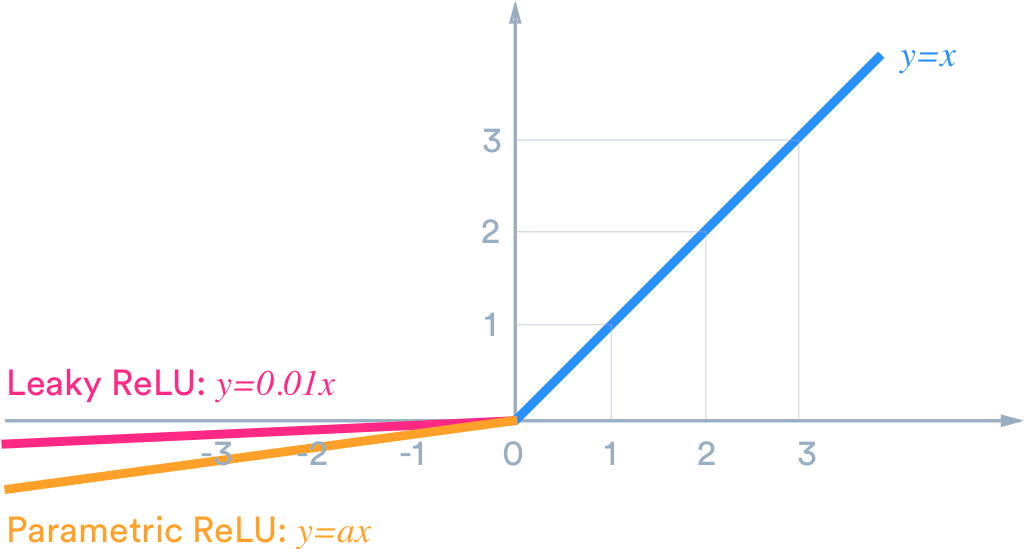
\includegraphics[width=80mm]{Images/LeakyRELU.png}   
\end{center}
\medskip

There is consensus that RELUs are much better (and faster) than
e.g. sigmoid-functions. There is no consensus about leaky RELUs.

\end{frame}


%-------------------------------------------------------------------
\begin{frame} 
\frametitle{Max-pooling}
For many purposes, a resolution given by the input image is not
needed. In object recognition an approximative position, size and
aspect ratio of a bounding box may suffice. \\[3mm]

To gather sufficient context information large filters are
needed. These cost a lot in the number of parameters. Instead
the images are downsampled (usually with a factor 2 in each
direction). This may take place repeatably after each RELU.
Thus the architecture becomes pyramid-like.  \\[3mm]

When four pixels are downsampled to one, a pooling operation must be
applied. Most often this is a maximum. 

\end{frame}



%-------------------------------------------------------------------
\begin{frame} 
\begin{center}
  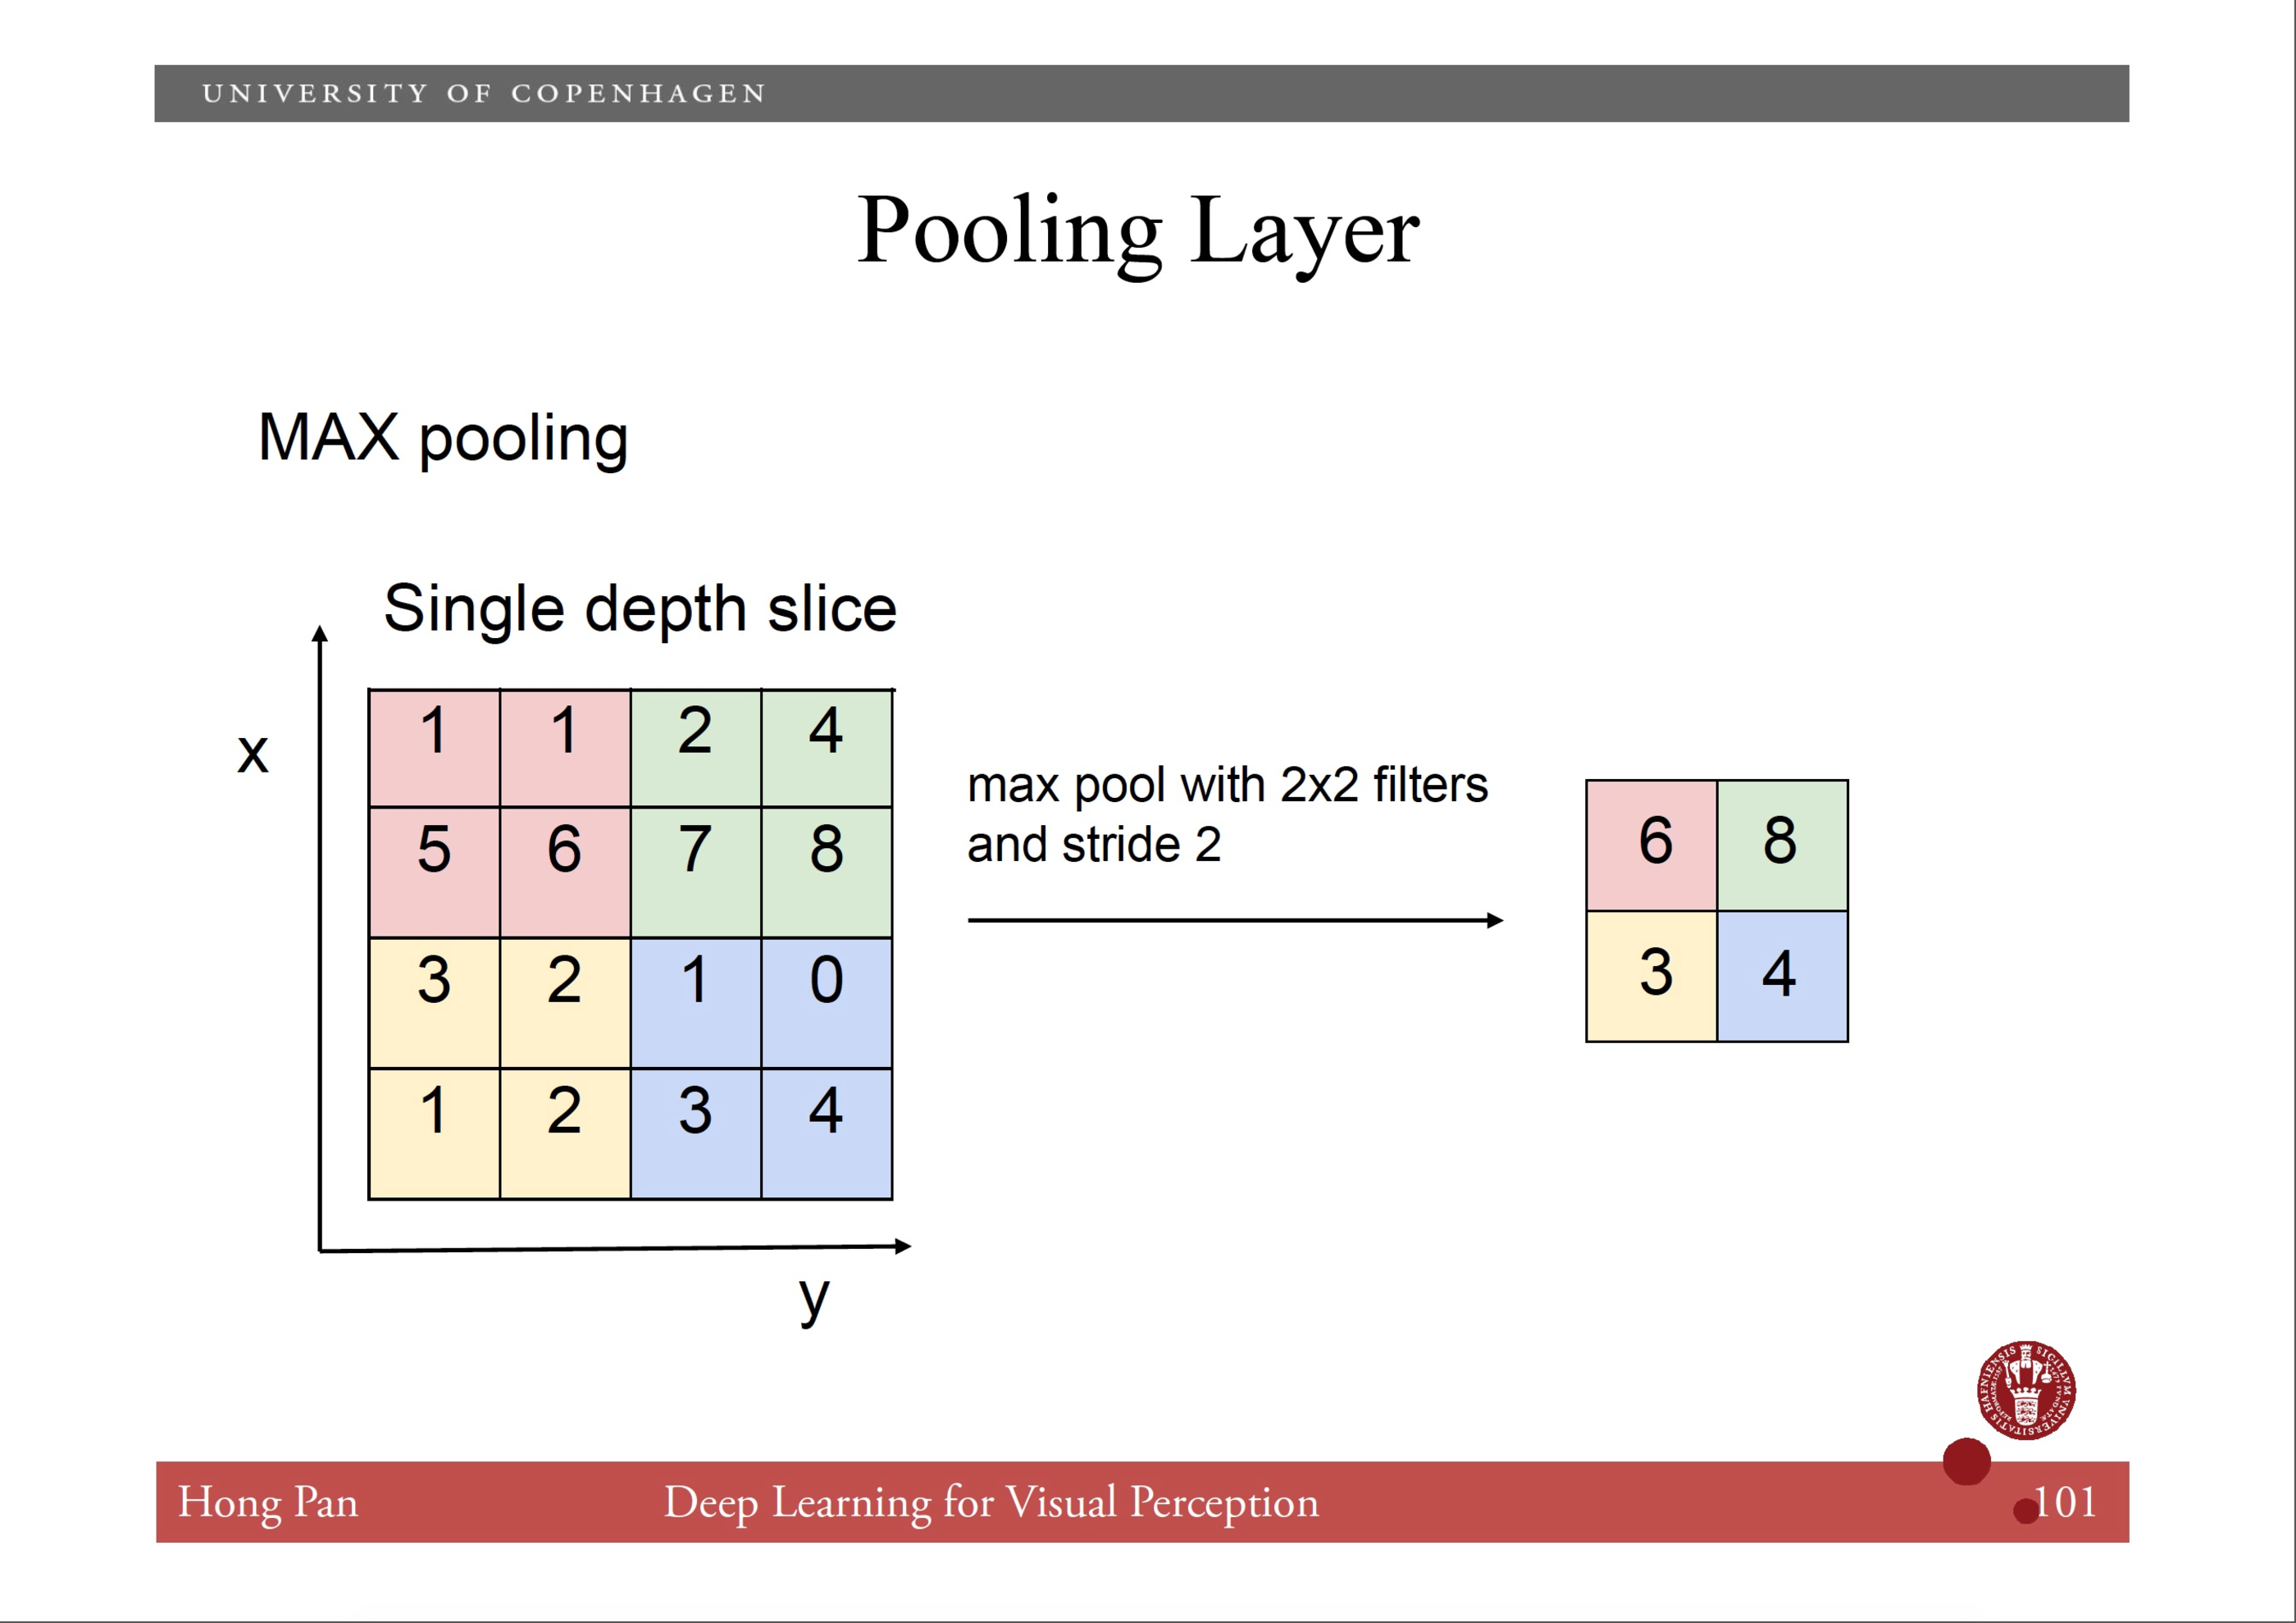
\includegraphics[width=120mm]{Images/pooling.pdf}   
\end{center}
\end{frame}



%-------------------------------------------------------------------
\begin{frame} 
  \frametitle{Average pooling}
  An average is a linear operation and does not provide the
  non-linearity often needed in learning processes.  However, in
  applications where counting/integration is essential, average
  pooling is possible. \\[4mm]

  \begin{center}
  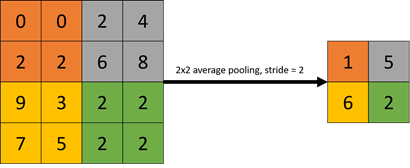
\includegraphics[width=100mm]{Images/averagePooling.png}   
\end{center}

\end{frame}



%-------------------------------------------------------------------
\begin{frame} 
  \vspace{15mm}

  \begin{center}
    {\color{blue}{\huge Questions ?}} \\[4mm]
%     {\huge Pause 10 minutes}
      \end{center}
\end{frame}



%-------------------------------------------------------------------
\begin{frame} 
\frametitle{Other layer types}
In object recognition, the last 1-3 layers are {\color{blue}{fully connected (FC)}}.
This part of the netork thus resembles a traditional neural net, and often
accounts for half the number of parameters (or more). \\[3mm]

Another usefull layer type performs normalization
({\color{blue}{NORM}}). This may be done
in many ways - one is to make sure all channels contribute with equal
amount to the following layer. \\[3mm]

Finally, to stabilize the learning of the FC-layers, often a
{\color{blue}{DROPOUT}} layer is used. During training, this
temporarily disconnects say half the neurons from
contributing. DROPOUT was used a lot in early nets. 
Later architectures prefer {\color{blue}{BATCH-NORMALIZATION}}. \\[3mm]

At the very end/top of most CNN's {\color{blue}{SOFTMAX}}-layers,
{\color{blue}{CLASSIFICATION}}-layers, or
{\color{blue}{REGRESSION}}-layers are usually applied. We 
will not discuss those layer types here.

\end{frame}




%-------------------------------------------------------------------
\begin{frame}
  \frametitle{Batch normalization}
  The purpose of Batch Normalization is to perform regularization.
  For each channel, it simply subtracts the mean and divides by the
  standard deviation. \\[3mm]

  \begin{displaymath}
    BN_{\gamma, \beta} (x_l) \;=\;
    \gamma \; \left [\frac{x_l \;-\; \mu_B}{\sqrt{\sigma_B^2 + \epsilon}}
      \right ]      \;+\; \beta
    \end{displaymath}
    where $(\gamma, \beta)$ are papameters that in the simple case may
    be $(1,0)$, but otherwise are trainable. \\[3mm]

    Batch Normaliztion may often be applied immediately after all
    (or selected) convolutions. 
    
\end{frame}



%-------------------------------------------------------------------
\begin{frame} 
\begin{center}
  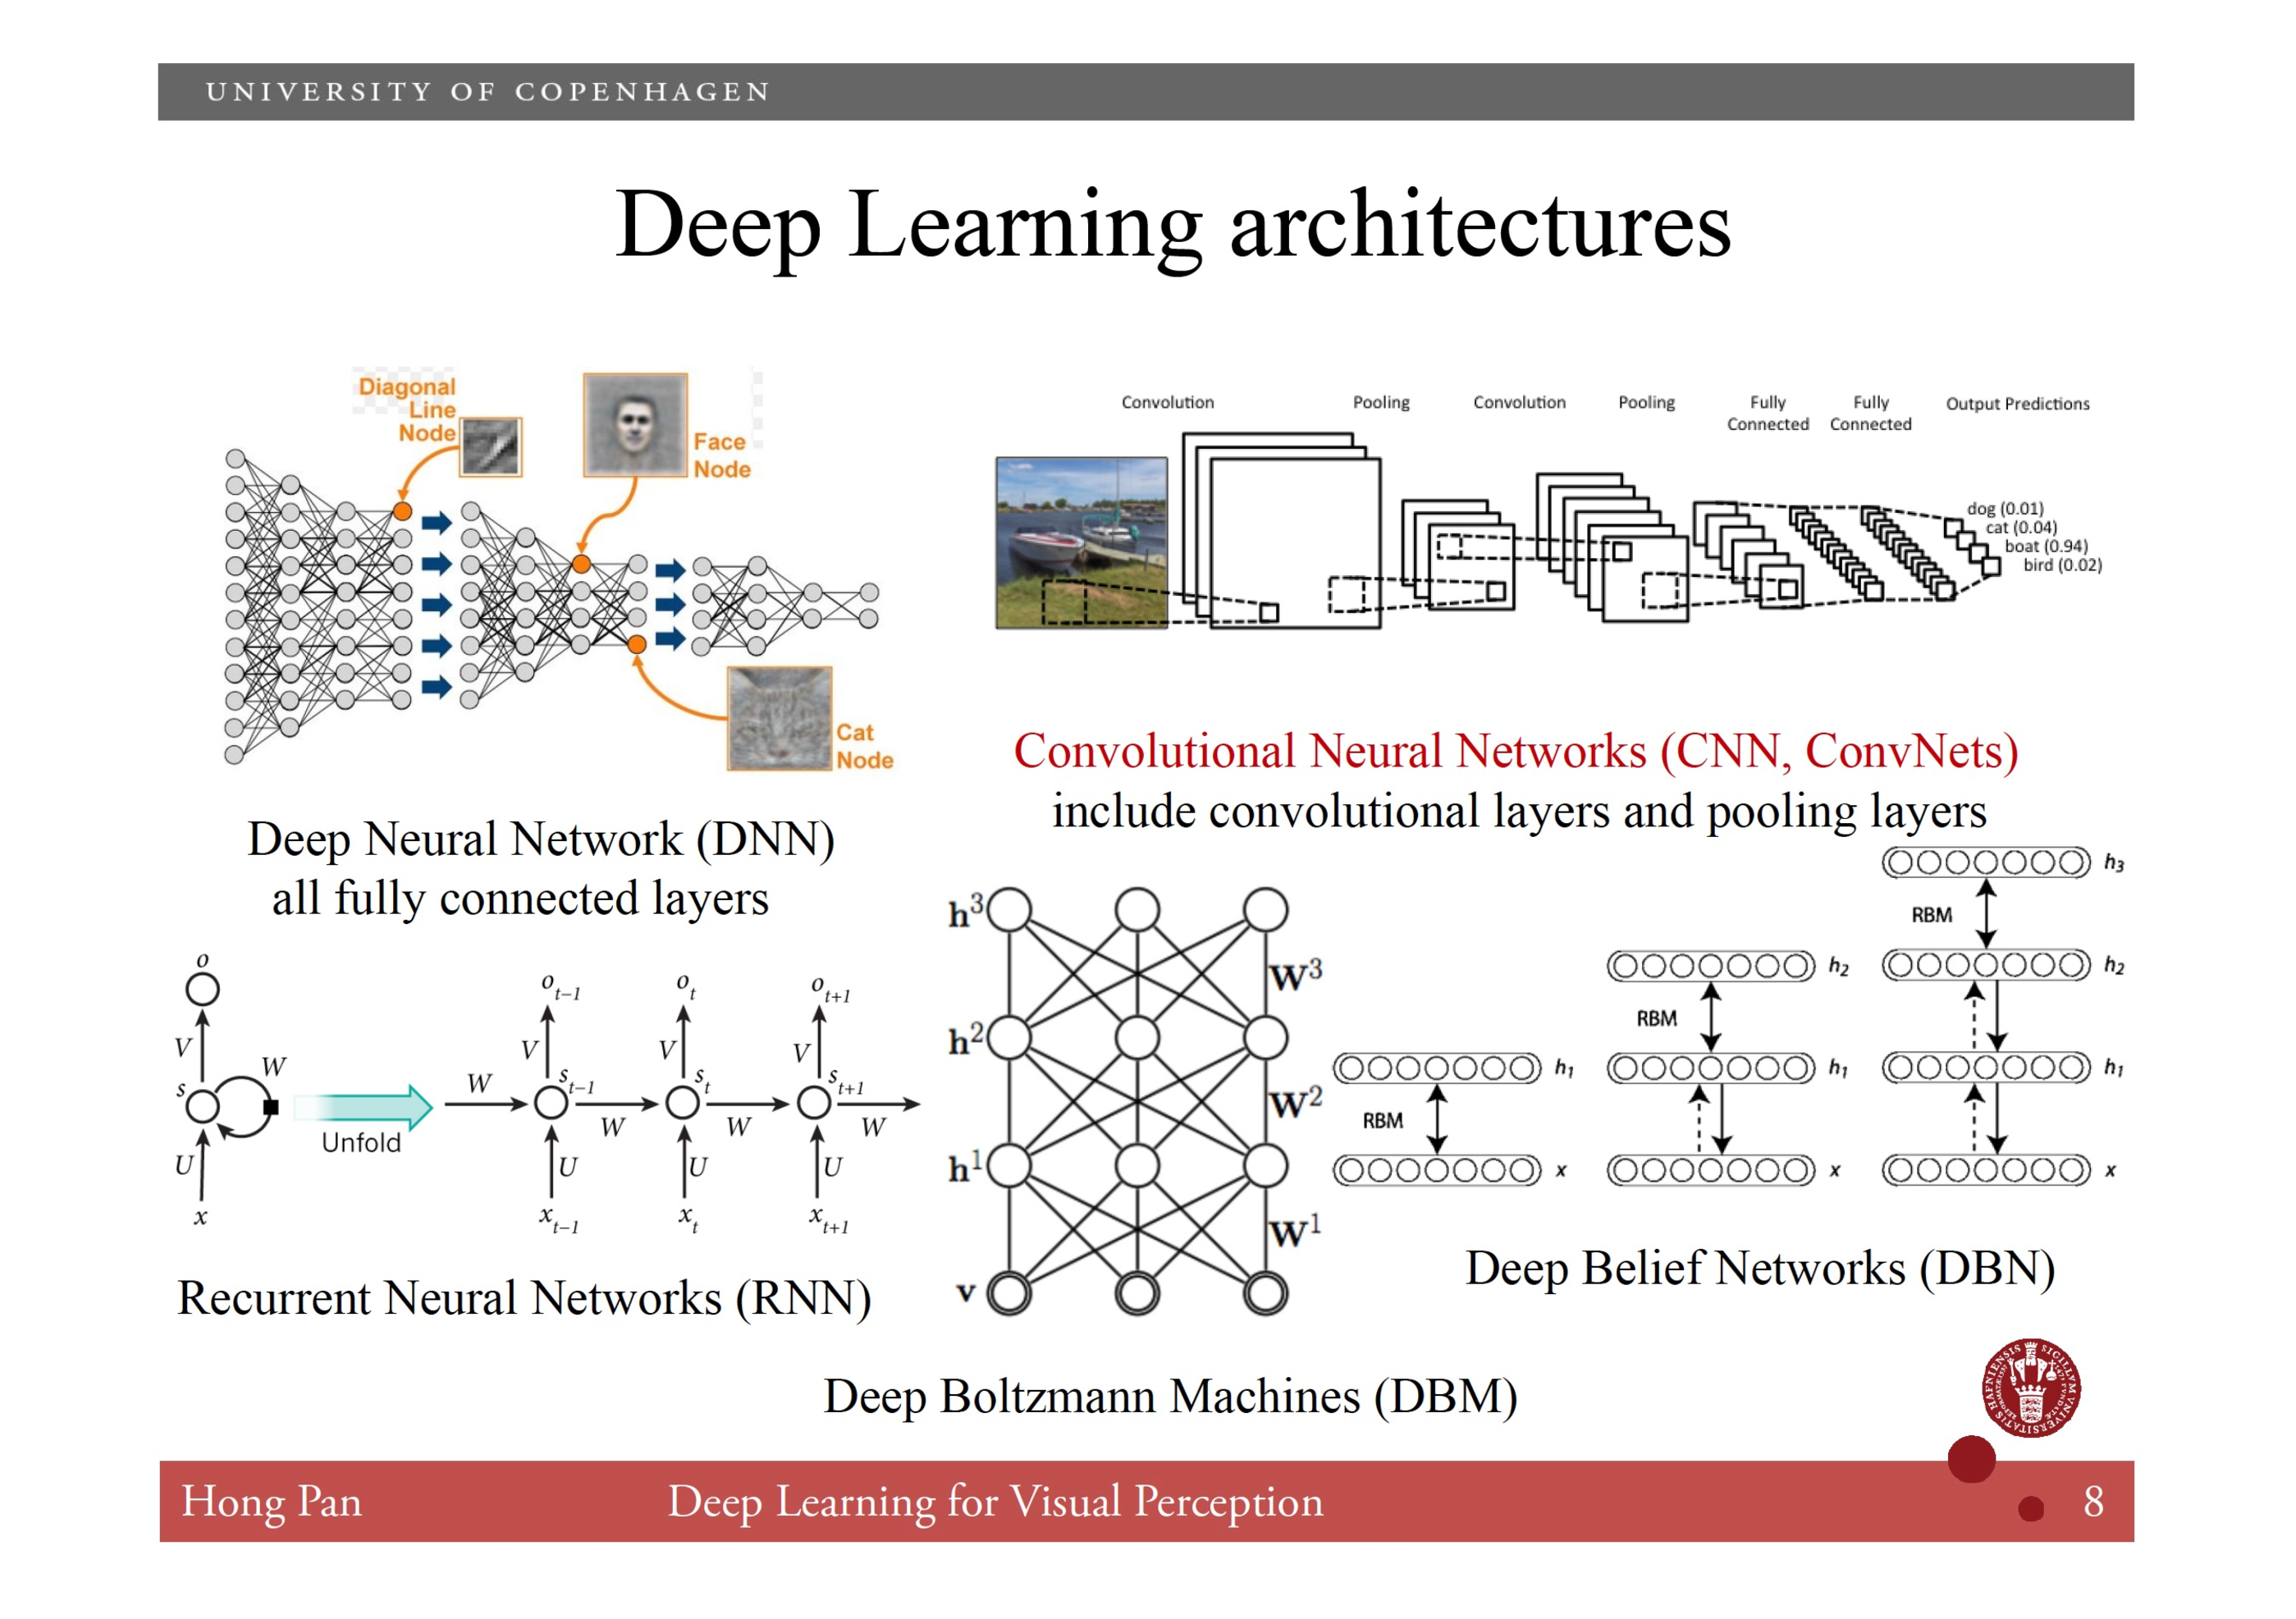
\includegraphics[width=120mm]{Images/Architectures1.pdf}
\end{center}
\end{frame}



%-------------------------------------------------------------------
\begin{frame} 
  \frametitle{It's so deep}

  {\color{red}{Deep Learning}} is a name for methods that decompose
  the input in a hierarchy of gradually more abstract
  representations. \\[4mm]

  Deep learning, like {\color{blue}{Neural Nets}} is a more general
  term than CNN.  It does not specify neither architecture, nor
  learning algorithm. \\[4mm]

  In the early 2010'ies, 5 levels were considered deep. Today this
  will be shallow.  Modern nets often applies 100 layers or more.
  However, increased depth does not necessarily imply increased
  performance. 
  
\end{frame}



%-------------------------------------------------------------------
\begin{frame} 
\frametitle{Putting it all together}
Many CNN's are build using a set of fixed layers, here called a 
{\bf level}. As example, we may construct a level by two 
$3 \times 3 \times k$ CONV layers, a RELU and a MAXPOOL layer. \\[5mm]

Two $3 \times 3$ convolutions could as well be implemented using one 
$5 \times 5$ convolution, but the former use only 18 parameter where
the latter use 25, an important saving. Modern CNN's tend to apply $3
\times 3$ CONV's only. \\[5mm]

Now stacking a number of levels and adding a FC creates a simple CNN.
\end{frame}



%-------------------------------------------------------------------
\begin{frame} 
\frametitle{What is going on?}
The purpose of the CONV-layers is to do feature extraction.  Going up
the levels gradually more and more abstract feature maps are
build. Finally, classification may be done using af FC-layer. \\[5mm]

A CNN may specialize the features to the task represented by the
annotated images. This may involve a mix of texture and structural
elements, that are not obvious to humans. \\[5mm]

In certain restricted application areas, well-trained CNN's have
outperformed humans. In other tasks they lack behind, and even the
best CNN can only handle what it has been trained to.
\end{frame}



%-------------------------------------------------------------------
\begin{frame} 
\frametitle{CNN's}
In general the CNN-architecture should be constructed according to the
task that it is supposed to solve.  Early nets, like
{\color{blue}{Alex net}} are rather complicated and involves many
parameters (60 Million for Alex Net).

\begin{center}
  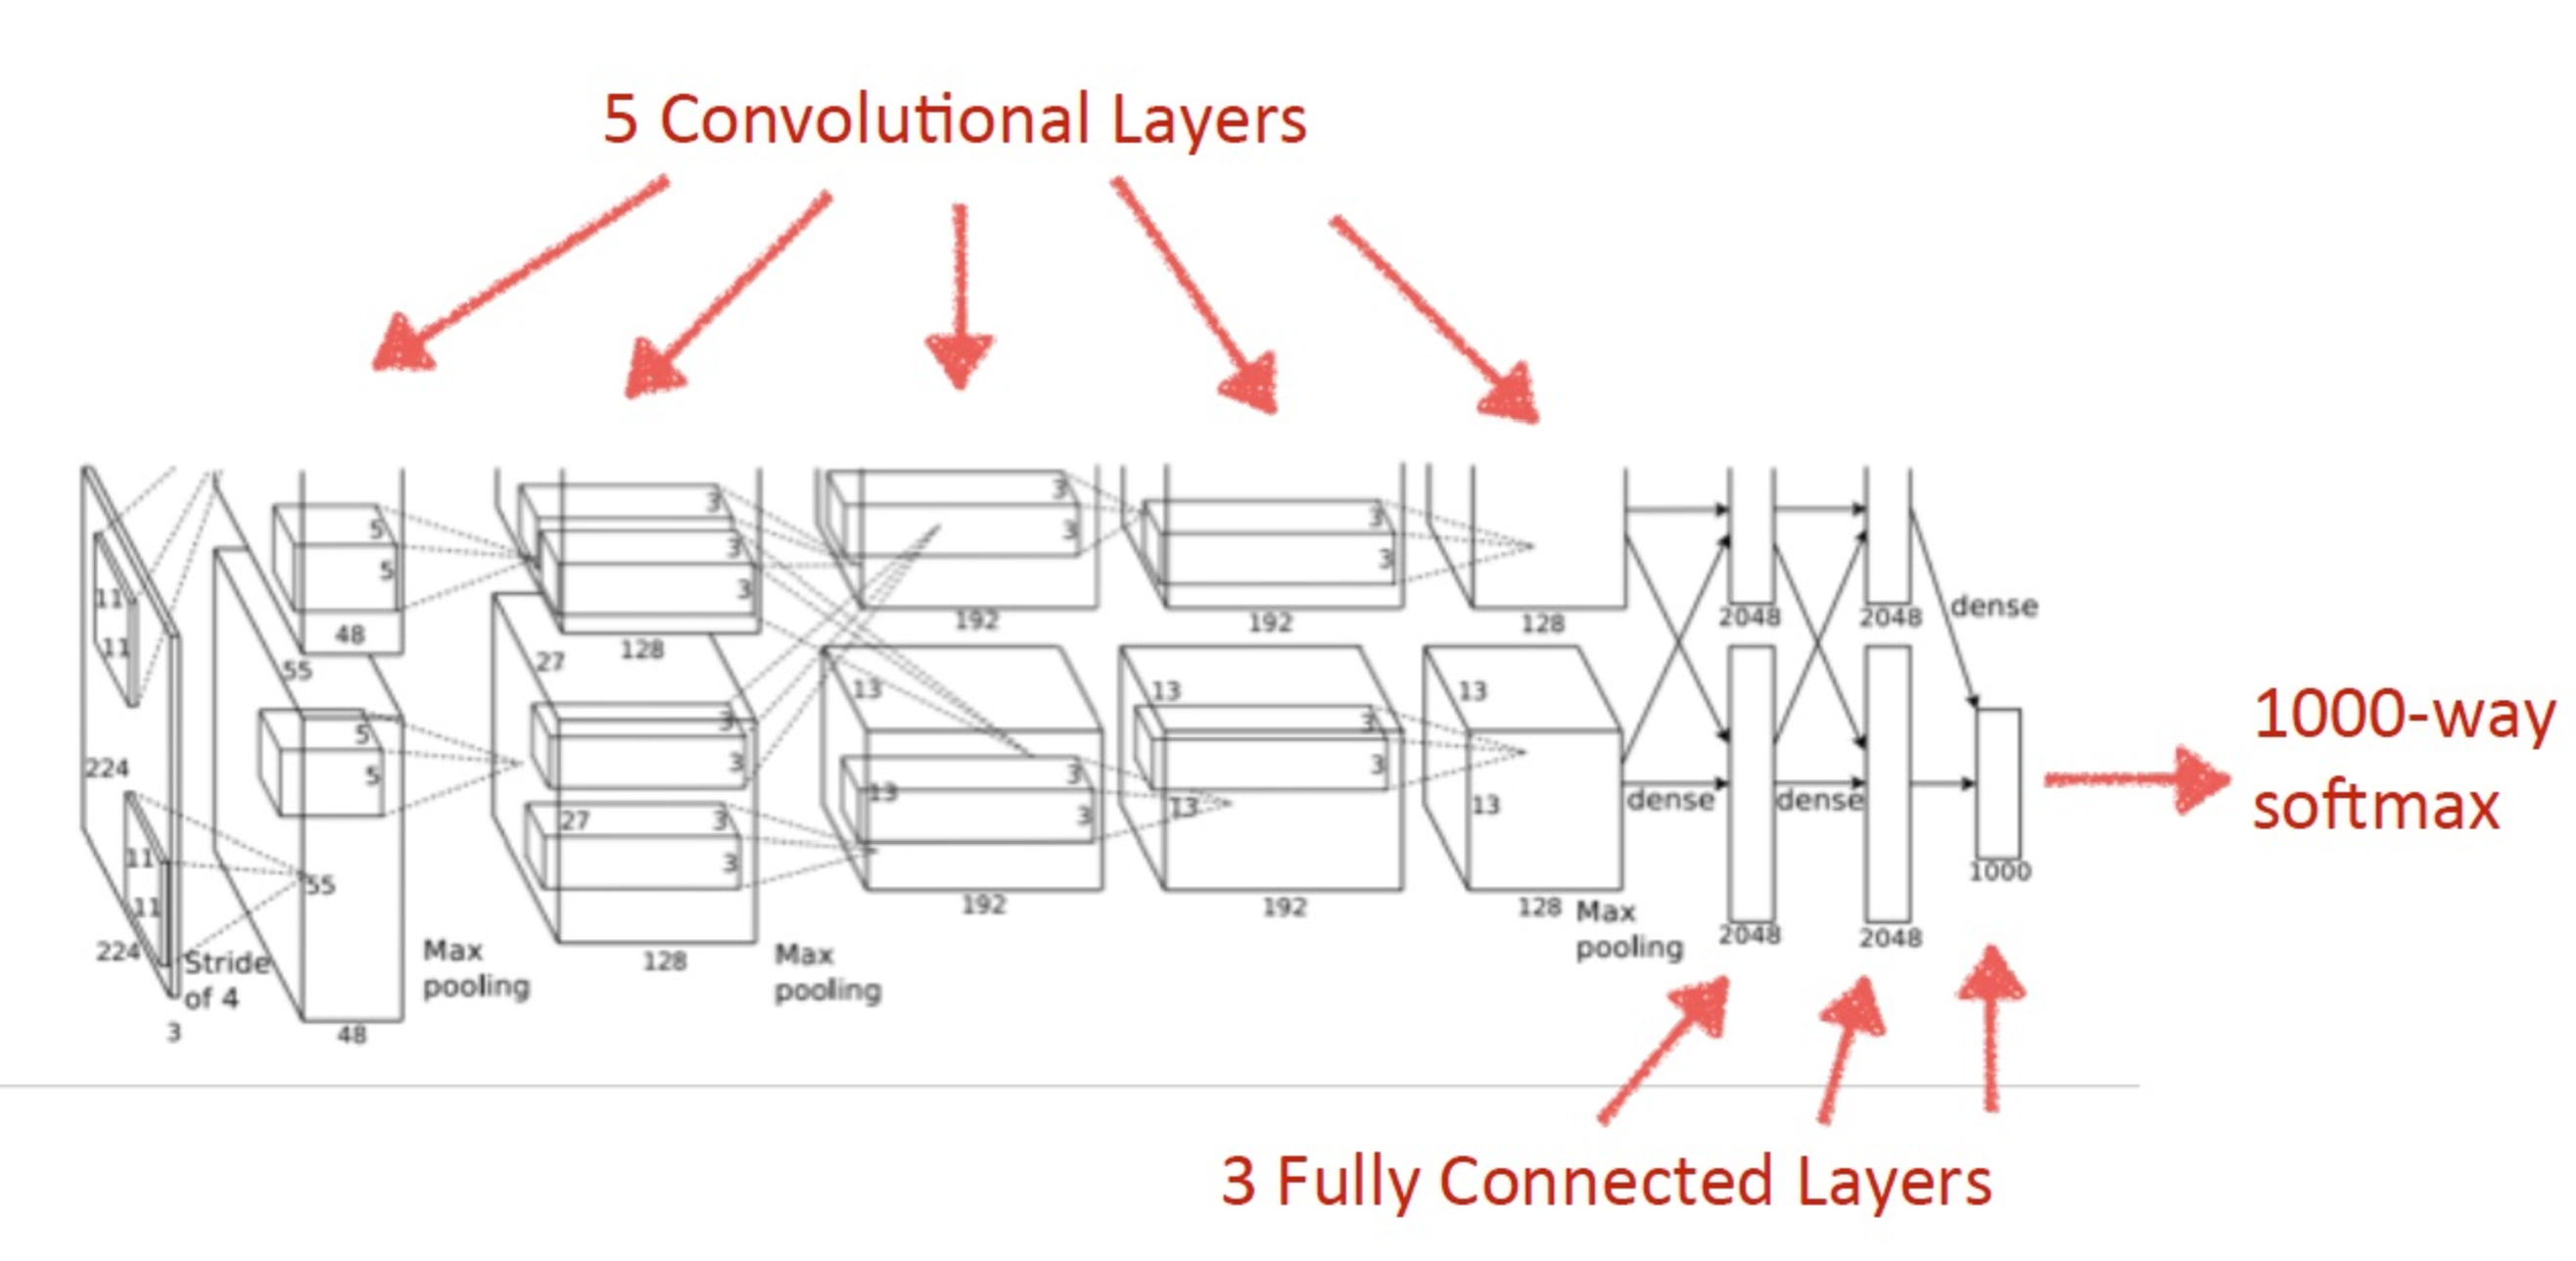
\includegraphics[width=110mm]{Images/AlexNet.pdf}   
\end{center}

Recent nets try to simplify and cut down the number of parameters.
\end{frame}



%-------------------------------------------------------------------
\begin{frame} 
\frametitle{Class exercise - 0.5 minute}
\vspace{1cm}
{\Large Where in AlexNet (or many other nets) do you think that the
  major number of parameters are used ?}   

\end{frame}




%-------------------------------------------------------------------
\begin{frame} 
\frametitle{A simple CNN}
Assume the Input size is $N \times N\times 3$:

{\tiny
\begin{center}
\begin{tabular}{l l l l} 
level & operation & filter size & output sixe\\
 1     &  Conv        & $3 \times 3\times 4$   & $N \times N\times 4$ \\
        &  Conv        & $3 \times 3\times 8$   & $N \times N\times 8$ \\
        &  RELU        &                                      & $N \times N\times 8$\\
        &  MAXPOOL & $2 \times 2$                &  $N/2\times N/2 \times 8$ \\
 2     &  Conv        & $3 \times 3\times 16$ & $N/2 \times N/2\times 16$ \\
        &  Conv        & $3 \times 3\times 32$ & $N/2 \times N/2\times 32$ \\
        &  RELU        &                                      & $N/2 \times N/2 \times 32$\\
        &  MAXPOOL & $2 \times 2$               &  $N/4 \times N/4 \times 32$\\
 3     &  Conv        & $3 \times 3\times 32$ & $N/4 \times N/4\times 32$ \\
        &  Conv        & $3 \times 3\times 64$  & $N/4 \times N/4\times 64$ \\
        &  RELU        &                                     & $N/4 \times N/4\times 64$ \\
        &  MAXPOOL &  $2 \times 2$              & $N/8 \times N/8\times 64$ \\
4     &  Conv         & $3 \times 3\times 128$ & $N/8 \times N/8\times 128$ \\
        &  Conv         & $3 \times 3\times 128$ & $N/8 \times N/8\times 128$ \\
        &  RELU         &                                  & $N/8 \times N/8\times 128$ \\
        &  MAXPOOL  & $2 \times 2$            & $N/16 \times N/16 \times 128$ \\
 5     &  DROPOUT  &                                 & $N/16  \times N/16 \times 128$ \\
        &  FC             & $M$                          & M \\
        &  FC             & $K$                           & K \\
        &  SOFTMAX  &                                  & K \\
        &  CLASSIFICATION &                        & 1 
\end{tabular}
\end{center}
}

Please note that only the CONV-layers and the FC-layers require
parameters that must be found during training.  Only the FC-layers
depend on the image size N. Now lets count the number of parameters.
\end{frame}



%-------------------------------------------------------------------
\begin{frame} 
\frametitle{Number of parameters}
Say we have $K$ classes and $M$ neurons in first FC-layer


\begin{center}
\begin{tabular}{l l l l} 
level & operation & filter size & parameters\\
 1     &  Conv        & $3 \times 3\times 4$ & $4*3*3*3 = 112$ \\
        &  Conv        & $3 \times 3\times 8$ & $8*3*3*4 = 288$ \\
 2     &  Conv        & $3 \times 3\times 16$ & $16*3*3*8 = 1152$ \\
        &  Conv        & $3 \times 3\times 32$ & $32*3*3*16 = 4608$ \\
 3     &  Conv        & $3 \times 3\times 32$ & $64*3*3*32 = 18.432$\\
        &  Conv        & $3 \times 3\times 64$ & $64*3*3*64 = 36.864$ \\
4      &  Conv         & $3 \times 3\times 128$ & $128*3*3*64 = 73.728$ \\
        &  Conv         & $3 \times 3\times 128$ & $128*3*3*128 = 147.456$\\
 5     &  FC             & $M$ & $(N/16)^2*128*M = N^2*M/2$ \\
        &  FC             & $K$ & $K*M$ \\
\end{tabular}
\end{center}

Feature levels contribute with a total of $282.640$ parameters.
Say $N = 200$ (small image patches), $K = 10$, and $M = 100$, then FC-layers
amounts to $2.000.000 + 1000 = 2.001.000$ parameters.

So in total we have about $2.28$ M parameters where the FC-layers are
responsible for most. To estimate all those parameters we need
efficient machine learning and {\bf a lot of data}.
\end{frame}



%-------------------------------------------------------------------
\begin{frame} 
  \frametitle{VGG-net}
  VGG won the ILSVRG (Image Net Large Scale Visual Recognition
  Competition) in 2014. It has later been made popular in a range of
  variants (VGG11, VVG16, VGG19).

\begin{center}
  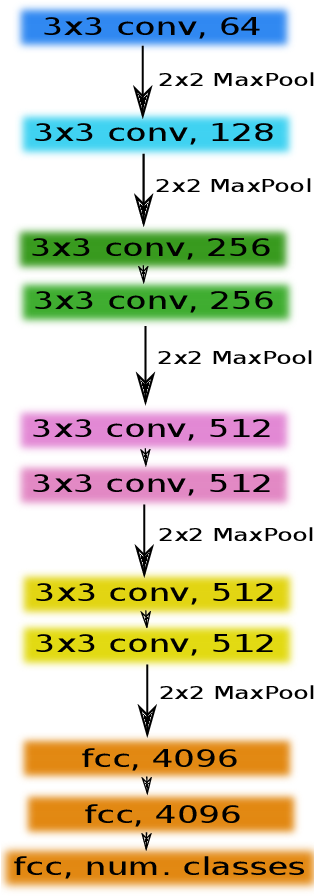
\includegraphics[width=20mm]{Images/VGG11.png}   
\end{center}

\end{frame}



%-------------------------------------------------------------------
% \begin{frame} 
%  \vspace{15mm}
%
%   \begin{center}
%     {\color{blue}{\huge Questions ?}} \\[4mm]
%     {\huge Pause 10 minutes}
%       \end{center}
% \end{frame}


%-------------------------------------------------------------------
\begin{frame} 
\frametitle{The Image Size}

Note that in all CNN's the size of the input image is fixed. The size
determines the number of neurons in the FC-layers. \\[4mm]

Often context information (i.e. image size) is determining the
performance. In general, when enlarging image size, the CNN depth as
well as the number of channels should also be increased. \\[4mm]

Thus increasing image size, increases the number of parameters, making
learning harder and increases the risk of overfitting.

\end{frame}



%-------------------------------------------------------------------
\begin{frame} 

\begin{center}
  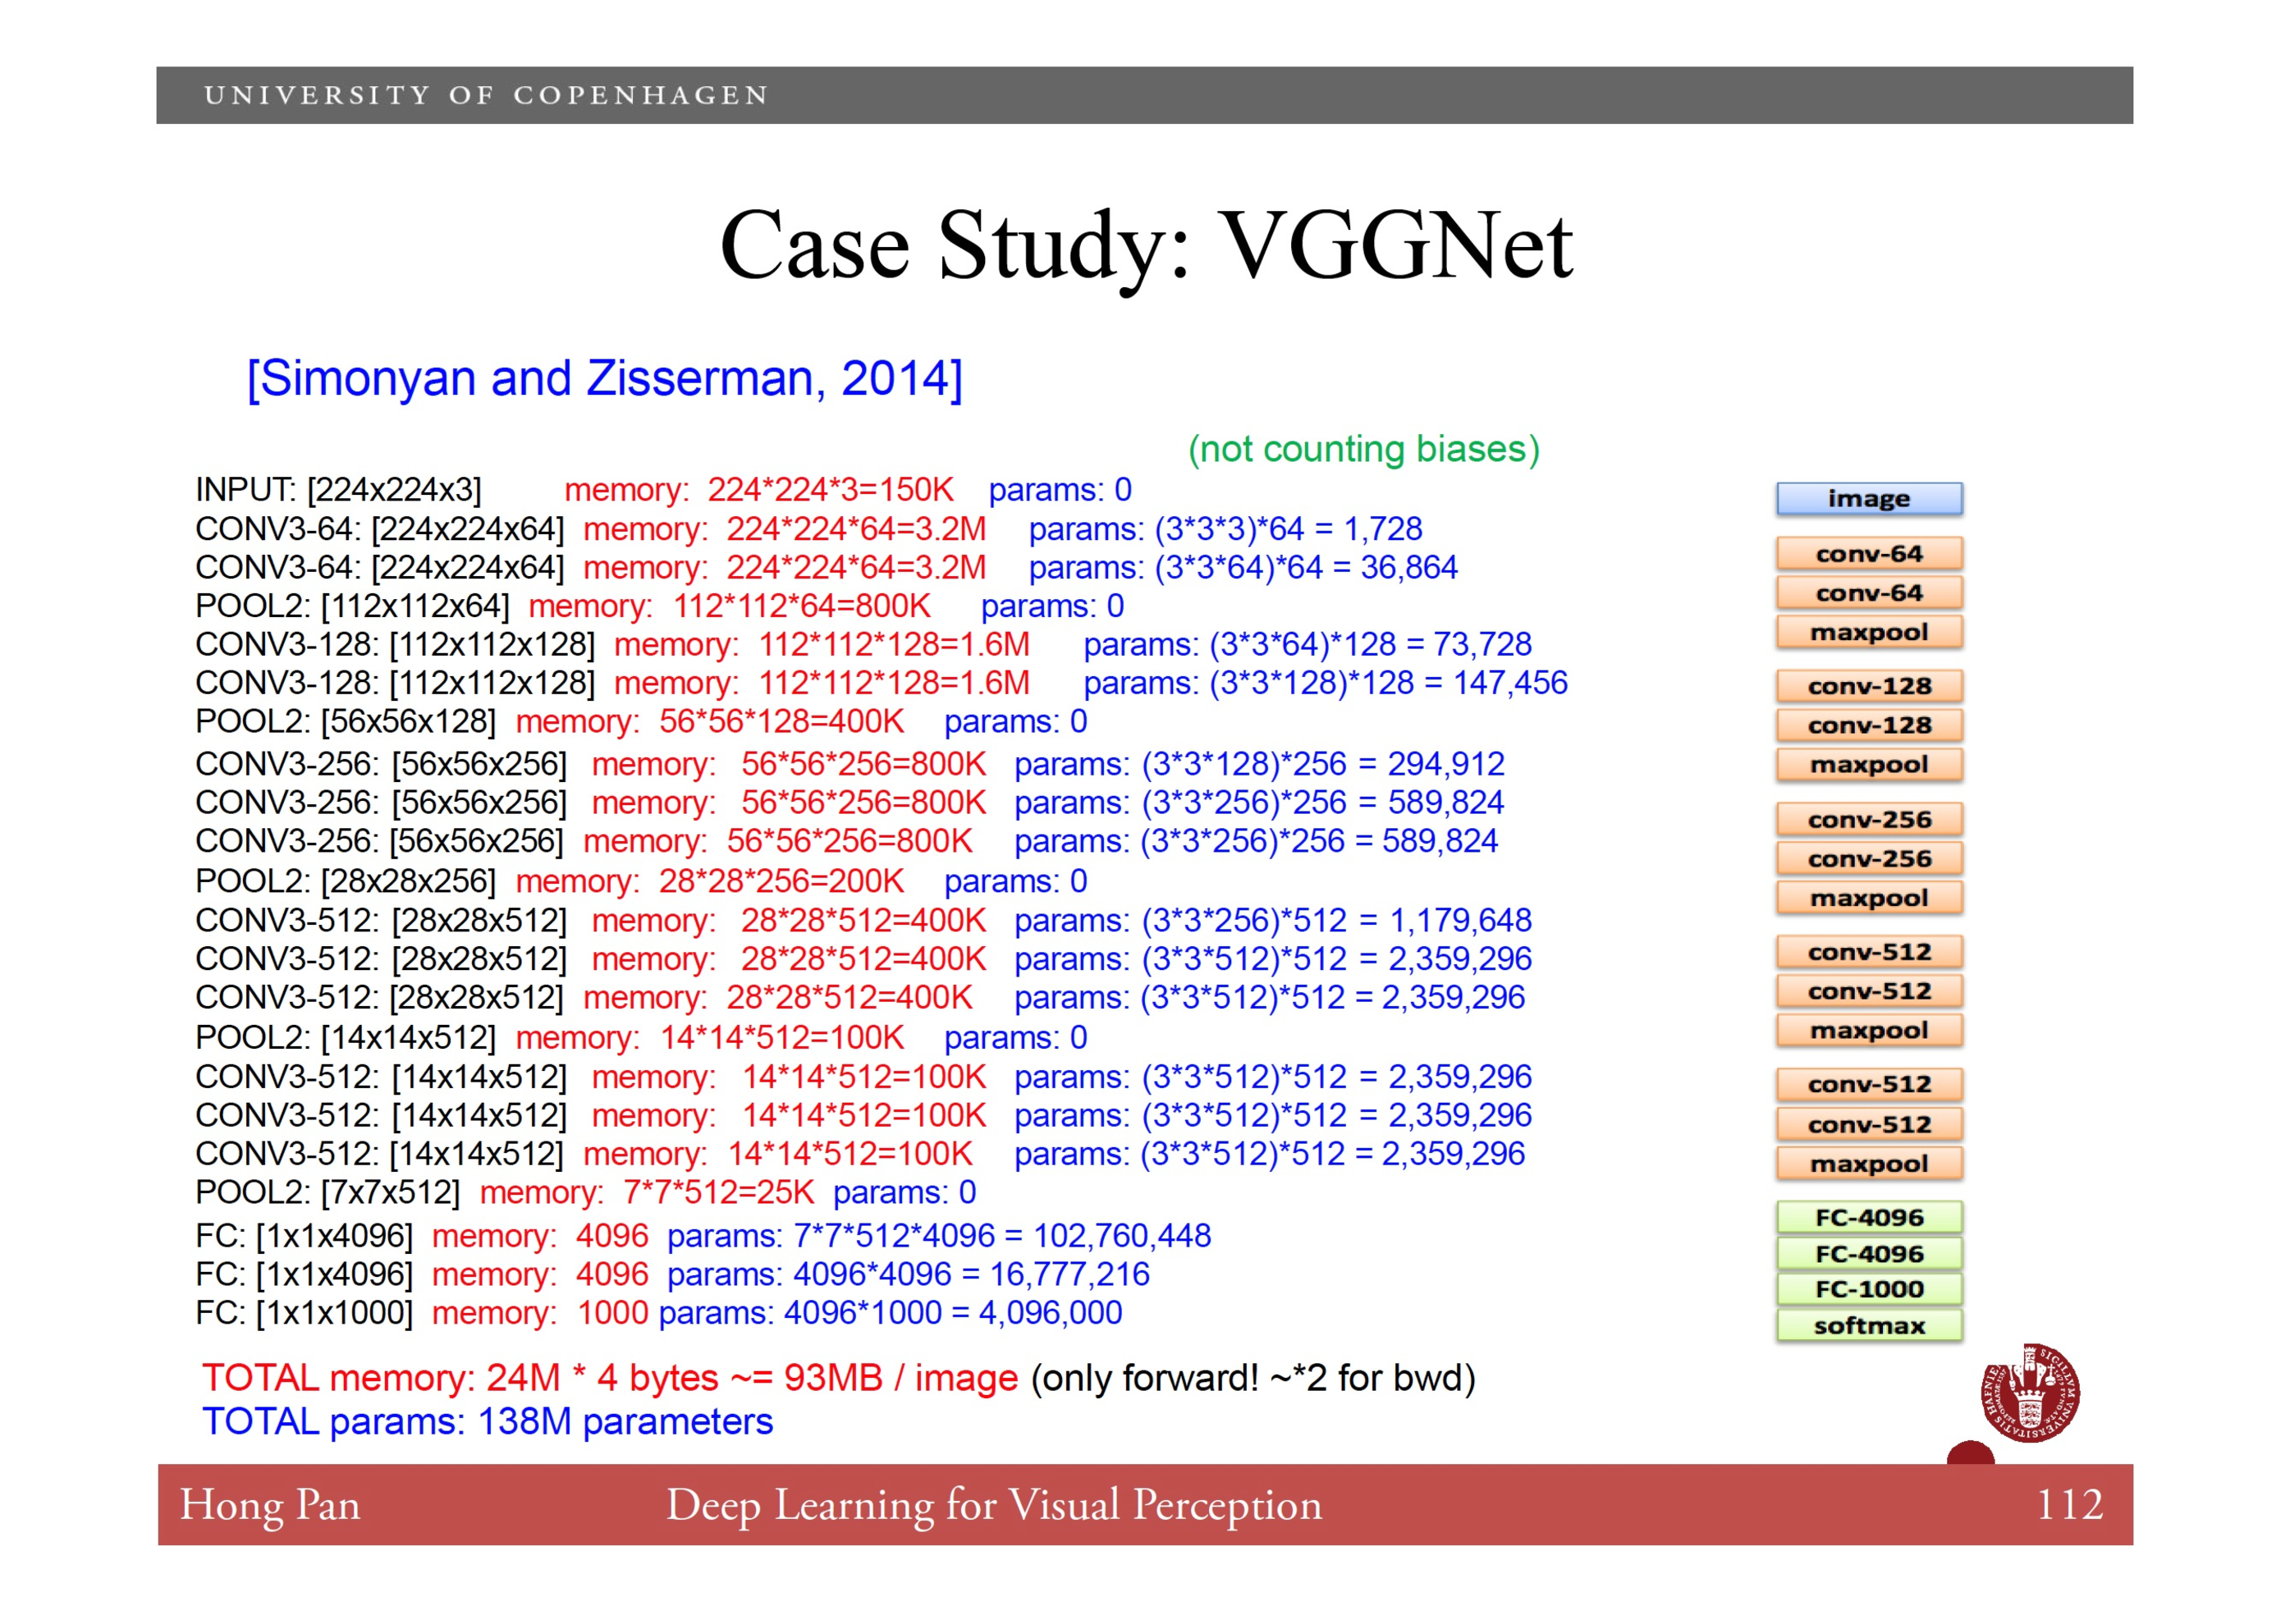
\includegraphics[width=120mm]{Images/VGGnet.pdf}   
\end{center}
\end{frame}


%-------------------------------------------------------------------
\begin{frame} 

\begin{center}
  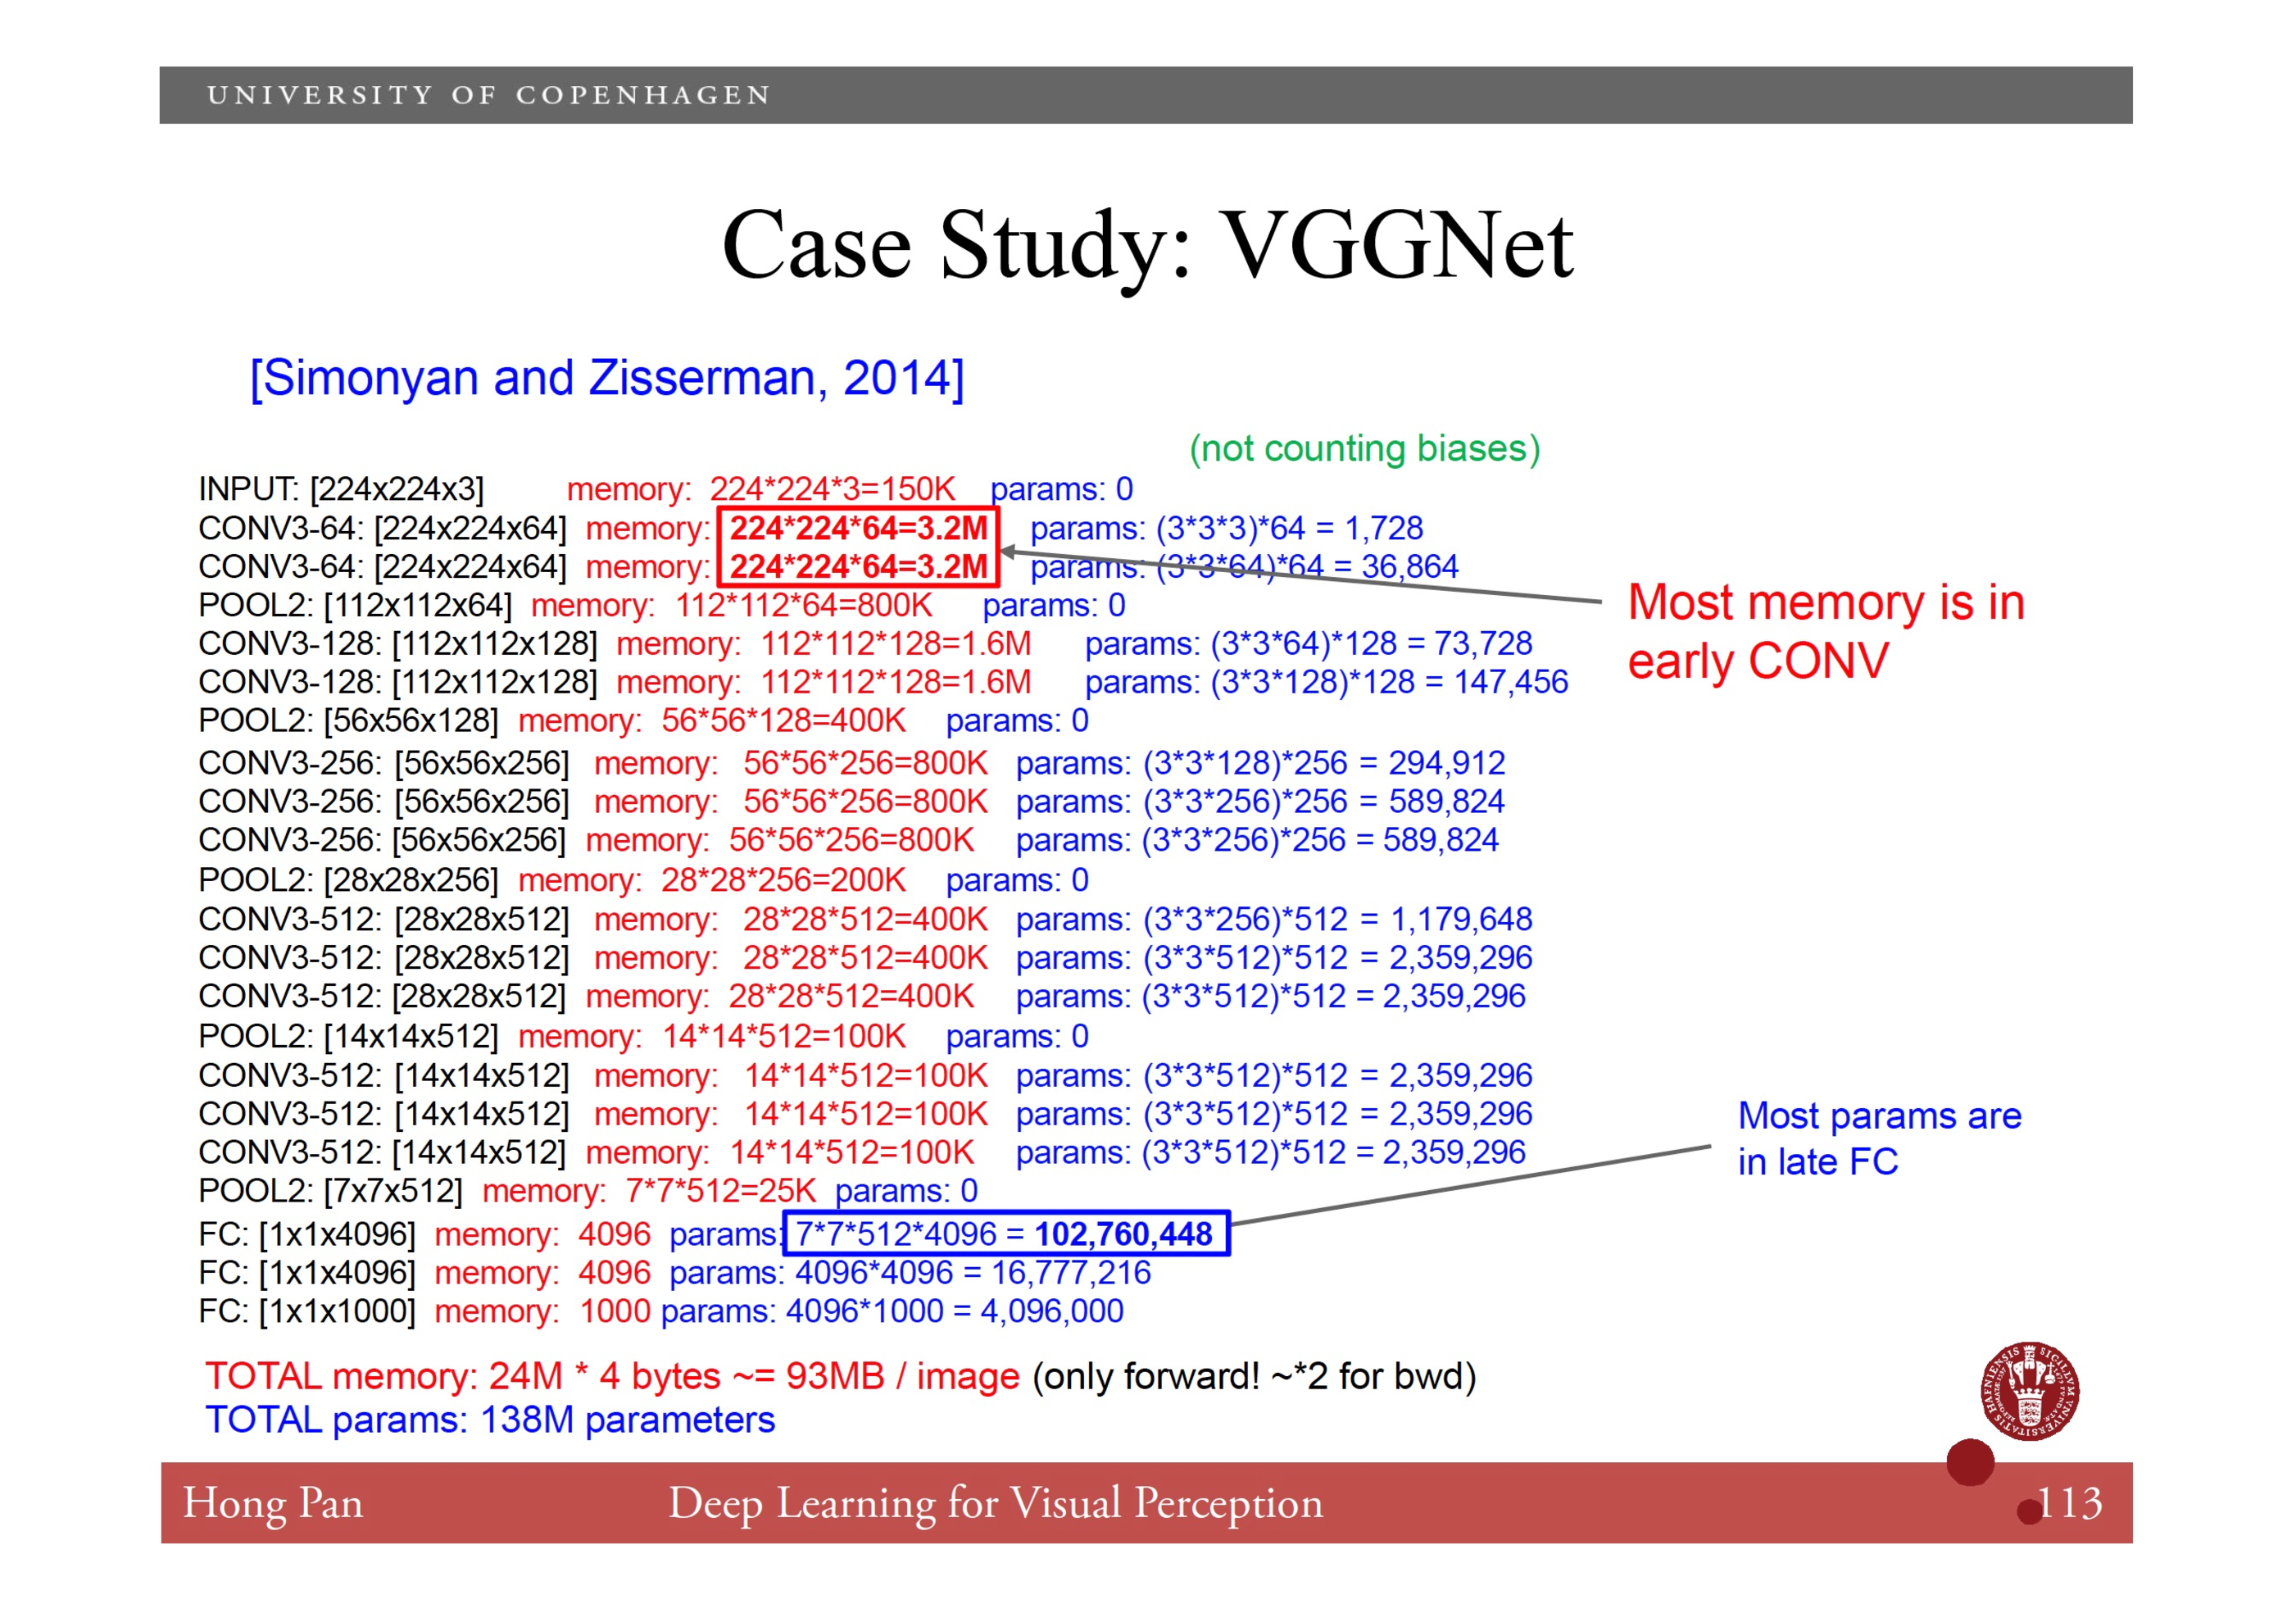
\includegraphics[width=120mm]{Images/VGGnet2.pdf}   
\end{center}
\end{frame}



%-------------------------------------------------------------------
\begin{frame} 
\frametitle{Modern CNN's}
The succes of AlexNet created a boost of research in particular within
CV.  Many far better nets have since 2012 been developed and the trend
continues.\\[4mm]

CNN's have shown superior in a number of areas including:
\begin{itemize}
\item Visual object recognition
\item Image segmentation and scene interpretation
\end{itemize}
\bigskip
 
CNN's are inappropriate when shift-invariance cannot be
assumed (and convolutions consequently does not apply). Also, they
require {\color{red}{\bf HUGE}} amounts of annotated data, access to
fast GPU's and days and weeks of training.
\end{frame}




%-------------------------------------------------------------------
% \begin{frame} 
% \frametitle{The future}
% In particular after 2016, {\color{blue}{Deep Neural Networks}} (CNNs)
% have been state-of-the-art in much Image Analysis and Computer
% Vision. \\[4mm]
%
% It is expected that the development will continue. In particular CNN's
% may find application in many industrial tasks, because now the
% performance has passed a threshold. \\[4mm]
%
% However, there will still exist plenty of areas where traditional IA
% and CV will be more appropriate.  \\[4mm]
%
% Also remember that if you don't know about filters, convolutions,
% linear algebra, fundamental matrices, epipolar lines, optical flow,
% etc. then access to a CNN will be of no use for you.
% \end{frame}



%-------------------------------------------------------------------
% \begin{frame} 
% \frametitle{Why you don't learn (more) about all this}
%
% \begin{itemize}
% \item You don't have the mathematical prerequisites.  \\[2mm]
% \item You don't have sufficient knowledge on numerical optimization.\\[2mm]
% \item We don't have time here to learn you what is needed. \\[2mm]
% \item It is difficult to design small exercises with limited amount of
%   data.\\[3mm]
% \item You don't have sufficient computer power.\\[2mm]
% \item You would learn very little, but waste a lot of time.
% \end{itemize}
% \bigskip
%
% In {\color{blue}{Advanced Topics in Image Analysis}} (ATIA), a thesis
% preparation course, CNN's will be treated in greater depth.
% \end{frame}



%-------------------------------------------------------------------
% \begin{frame} 
%   \frametitle{CNN in art}
%
%   And now to something funny: \\[3mm]
%  {\color{blue}{Do you think CNN's may be of use in art ?}} \\[8mm]
% 
%   The idea is to process two images, one for contents, and the other
%   for painting style.  Then combine the representations to create a new
%  image. \\[6mm]
%
%  We skip the details ...
% \end{frame}



%  Take png/jpg image of pdf-images using preview

%-------------------------------------------------------------------
\begin{frame} 
\frametitle{CNN in art 1}
\begin{center}
  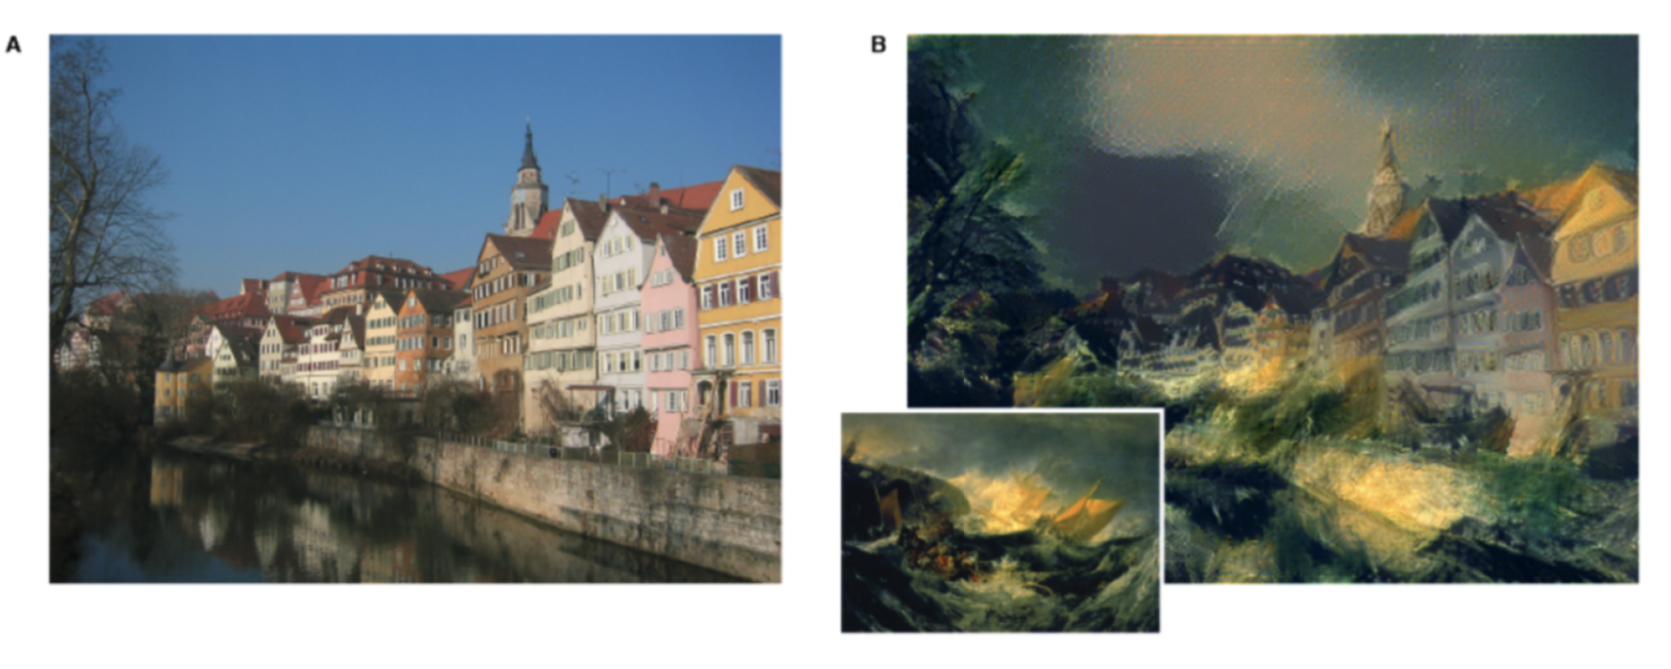
\includegraphics[width=100mm]{Images/art10.png}   
\end{center}
\end{frame}


%-------------------------------------------------------------------
\begin{frame} 
\frametitle{CNN in art 2}
\begin{center}
  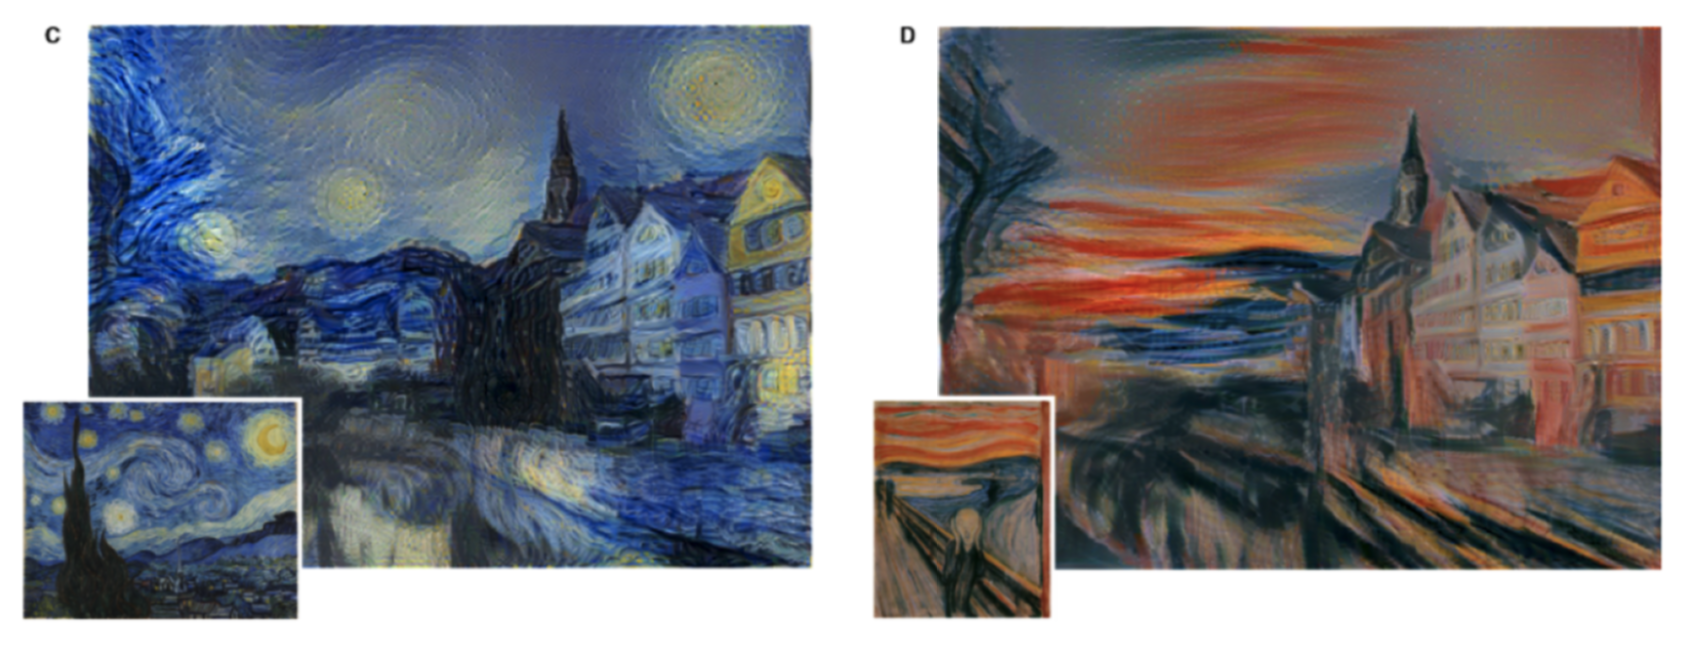
\includegraphics[width=100mm]{Images/art11.png}   
\end{center}
\end{frame}



%-------------------------------------------------------------------
\begin{frame} 
\frametitle{CNN for faking images}
\begin{center}
   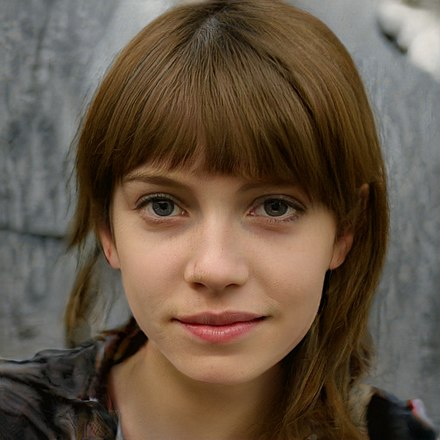
\includegraphics[width=50mm]{Images/GANfake.jpg}   
\end{center}
\end{frame}



%-------------------------------------------------------------------
\begin{frame} 
  \frametitle{Next time}
  \begin{itemize}
  \item What can a neuron compute ?
  \item Regularization, Optimization and  Loss functions
  \item Pretraining and transfer learning
  \item A gentle introduction to the zoo of network architecture
  \item A bit on object detection and image segmentation
  \item Course evaluation
  \end{itemize}
\end{frame}


\end{document}


